\chapter{ViDoRe v3 Appendix}


\section{Dataset examples}

\begin{figure*}[h]
    \centering
    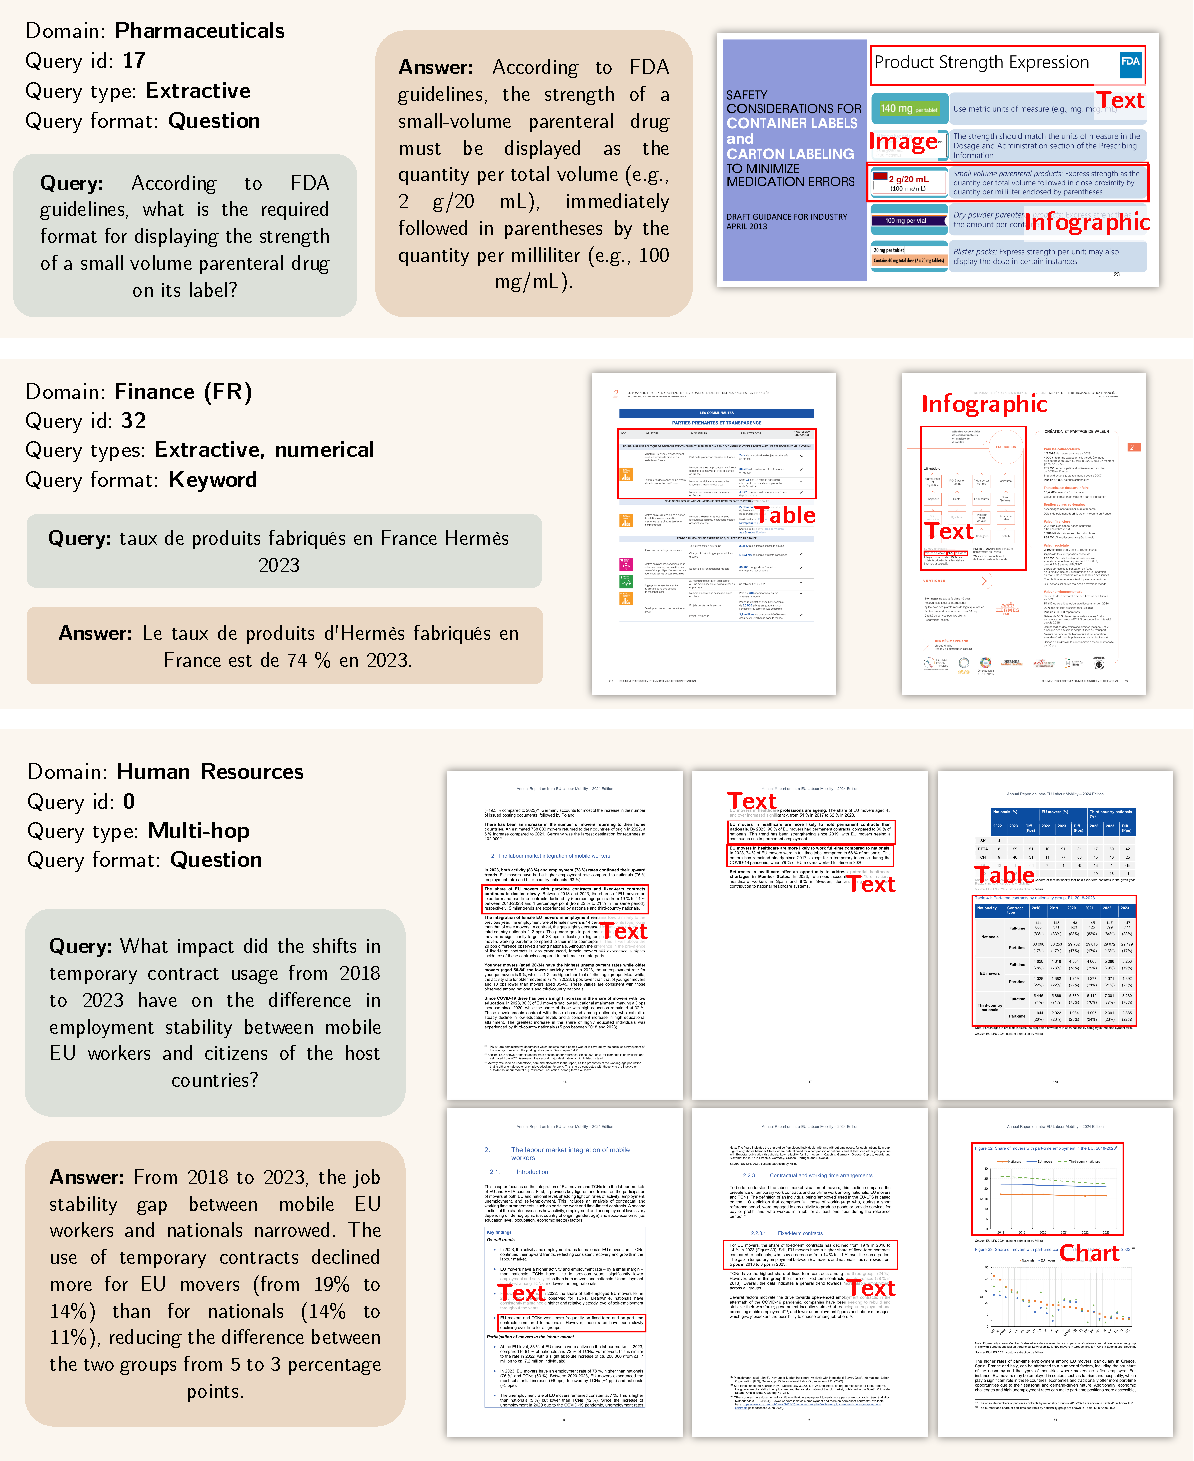
\includegraphics[width=0.92\textwidth]{images/vidorev3_images/dataset-examples.pdf}
    \caption{\textbf{Examples from the ViDoRe V3 datasets.} Featuring varied query types and visually rich document formats across multiple domains, the benchmark captures the complexity of real-world retrieval scenarios.}
\end{figure*}


\section{Supplementary benchmark details}

\paragraph{Domains} \Cref{tab:datasets} details the type of documents used in each corpus as well as several statistics.

\paragraph{Query type and format descriptions}

\Cref{tab:query_taxonomy} describes the types and formats of the queries, while \Cref{fig:upset plot} gives details about query type intersection frequency.

\paragraph{Query type by generation method}

Query type distributions by generation method (Figure~\ref{fig:query type by generation method}) confirm that open-ended queries dominate synthetic queries as the synthetic pipeline attributed more weight to this type, while extractive queries dominate human-image queries since they are more naturally chosen by annotators.

\section{Annotator pool and training details}
\label{appendix: annotator pool}
\paragraph{Annotator Pool and Selection.} Annotation was conducted by a curated pool of 76 annotators who were selected based on having: (1) a bachelor's degree or higher in the relevant domain, (2) professional experience in the domain, (3) native-level language proficiency as required by task, and (4) prior experience with RAG, retrieval, or VQA annotation projects. Quality control was performed by 13 senior annotators with enhanced domain knowledge and extensive annotation experience, with project oversight provided by data leads with multiple years of experience in human data generation.

\paragraph{Training and Pilot Phase.} The annotation process began with a comprehensive onboarding phase where annotators received task-specific training using gold-standard examples. For each domain, a pilot of several hundred tasks was conducted with 100\% quality control coverage and multiple annotators per task. During this phase, data leads and the research team continuously evaluated annotations, provided clarifications, and refined guidelines. Inter-annotator agreement and time-per-task baselines were calculated to establish ongoing evaluation benchmarks. The pilot concluded upon validation of both data quality and guideline effectiveness.

\section{Supplementary agreement metrics}
\label{appendix: relevance agreement}

Pages were pre-filtered by a VLM before human annotation; as most pages shown to annotators were likely relevant, this created a skewed class distribution. This prevalence imbalance causes traditional chance-corrected metrics like Krippendorff's Alpha to appear paradoxically low even when annotators genuinely agree, as inflated expected chance agreement penalizes the score. To address this, we report 2 complementary metrics: Krippendorff's Alpha (ordinal) as the standard measure and Gwet's AC2 which remains stable under prevalence skew. Overall, annotators achieved $\alpha = 0.469$, AC2 $= 0.760$. The divergence between Alpha and AC2/Weighted Agreement is expected given the pre-filtered data and confirms substantial agreement despite the skewed distribution.

\section{Supplementary retrieval details}
\label{appendix:supp retrieval}
\paragraph{Retriever model reference}

Table~\ref{tab:model_metadata} lists the retriever models evaluated in this work, along with their HuggingFace model names and citations.


\paragraph{Monolingual performance} \label{sec:english retrievers}

Tables~\ref{tab: english-only retrieval} and \ref{tab: french-only retrieval} present the monolingual performance of our models, where retrieval is conducted using language-matched queries and documents for English and French, respectively.

\begin{table*}[t!]
\centering
\small % Options: \small, \footnotesize (smaller), or \scriptsize (smallest)
\begin{tabularx}{\textwidth}{lXX} % 'l' for auto-width category, 'X' for wrapping columns
\toprule
\textbf{Category} & \textbf{Definition} & \textbf{Example} \\ \midrule
\multicolumn{3}{c}{\textit{\textbf{Query Types}}} \\ \midrule
\textbf{Open-ended} & Seeks explanatory or descriptive information that requires synthesis. & What drives the rise in women's workforce involvement in EU nations? \\
\textbf{Extractive} & Requires the retrieval of a specific piece of information. & Bank of America preferred stock MM dividend rate \\
\textbf{Compare Contrast} & Mandates a comparison between multiple entities or data points. & Explain the factors contributing to the reduction in R2R rates for ANDAs. \\
\textbf{Boolean} & Poses a yes/no question necessitating multi-step reasoning. & Did JPMorganChase execute more than half of its planned repurchase program? \\
\textbf{Numerical} & Asks for a specific quantitative value that must be derived or calculated. & percentage increase in Morgan Stanley revenue from 2023 to 2024 \\
\textbf{Multi-hop} & Requires integrating information from multiple sections or sources. & Summarize the steps involved in error reporting in ISMP's MERP. \\
\textbf{Enumerative} & Requests a list of all instances sharing a common property. & Specify the ISCO codes used to define domestic workers in the EU. \\ \midrule
\multicolumn{3}{c}{\textit{\textbf{Query Formats}}} \\ \midrule
\textbf{Question} & An interrogative sentence. & What was Citigroup's net interest margin in 2024? \\
\textbf{Keyword} & A non-verbal phrase or set of terms. & female employment rate European Union 2023 \\
\textbf{Instruction} & A directive specifying a task. & Identify the use case of a drill point gauge. \\ \bottomrule
\end{tabularx}
\caption{Taxonomy of Query Types and Formats.}
\label{tab:query_taxonomy}
\end{table*}

% \vspace{15cm}
% \hfill

\begin{figure*}[t!]
    \centering
    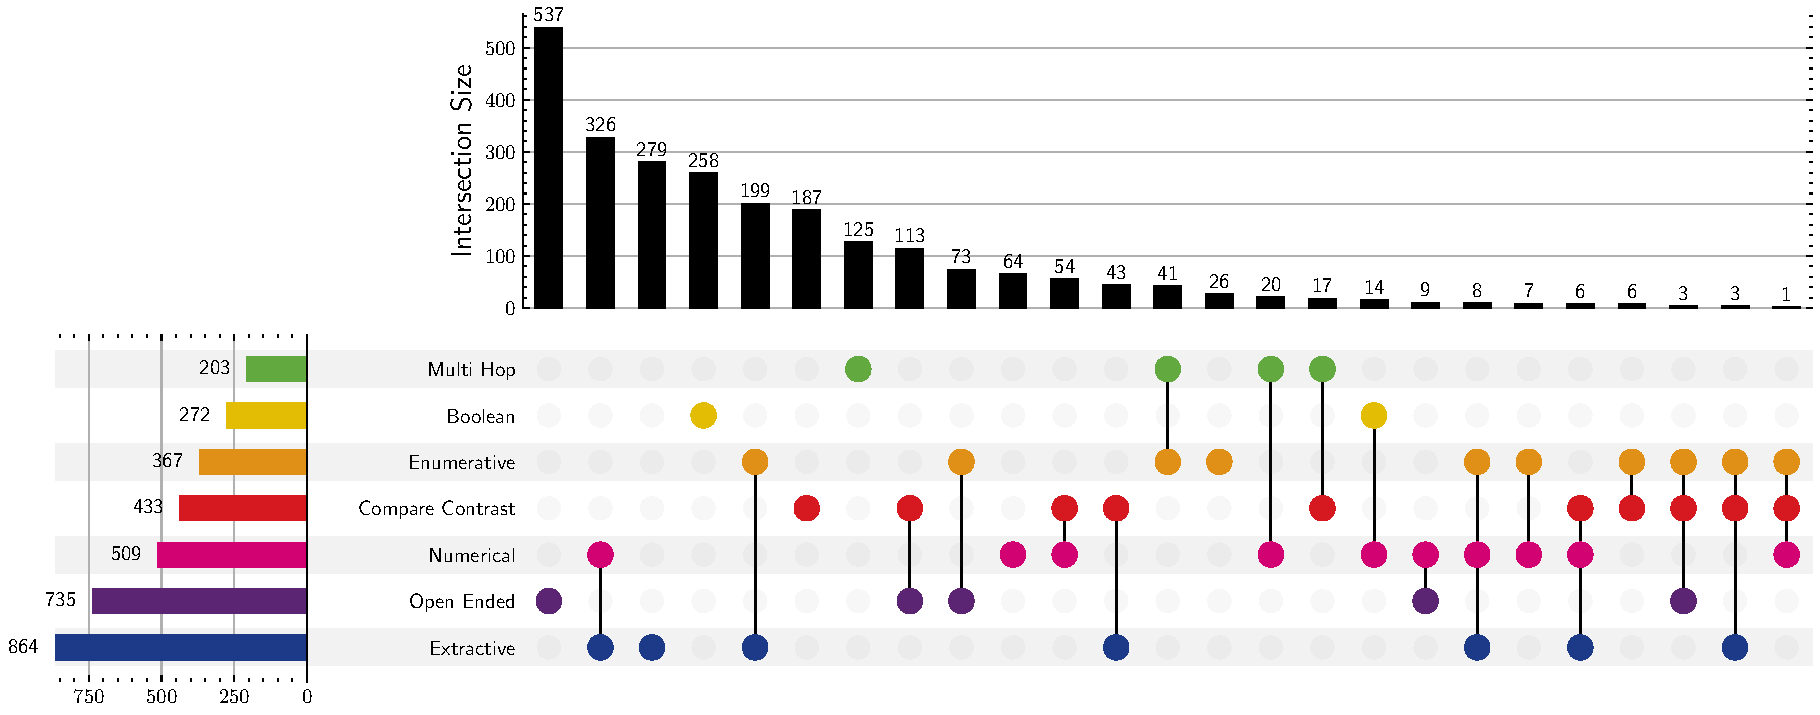
\includegraphics[width=\textwidth]{images/vidorev3_images/upset_plot_query_types_complete.pdf}
    \caption{\textbf{UpSet plot illustrating the distribution and intersection of query types in ViDoRe V3.} The horizontal bars on the left display the total count of queries for each individual type. The vertical bars at the top represent the frequency of specific combinations (intersections), as indicated by the connected dots in the matrix below. While \textit{Extractive} queries are the most prevalent overall, \textit{Open Ended} queries form the dominant unique category. Complex dependencies are evident in the frequent intersection of \textit{Enumerative} and \textit{Extractive types}, indicating a substantial subset of queries requiring list-based fact retrieval.} 
    \label{fig:upset plot}
\end{figure*}

% \clearpage

\begin{table*}[t]
\small
\centering
\setlength{\tabcolsep}{4pt}
\renewcommand{\arraystretch}{1.15}

\begin{tabularx}{\textwidth}{
    >{\RaggedRight\arraybackslash}X
    >{\RaggedRight\arraybackslash}X
    >{\RaggedRight\arraybackslash}p{4.2cm}
    c
    c
    c
    c
    >{\RaggedRight\arraybackslash}X
}
\toprule
\textbf{Corpus} &
\textbf{Domain(s)} &
\textbf{Description} &
\textbf{Lang.} &
\textbf{\# Docs} &
\textbf{\# Pages} &
\textbf{\# Queries$^{*}$} &
\textbf{Main modalities} \\
\midrule

\textbf{U.S. Public Company Annual Reports} &
Finance-EN &
Consists of 6 10-K annual reports from major U.S. financial institutions for the fiscal year ended December 31, 2024. &
en & 6 & 2942 & 309 &
Text, Table \\
\addlinespace

\textbf{Computer Science Textbooks} &
Computer Science / Education &
Consists of two open-source, peer-reviewed textbooks from OpenStax covering foundational topics in computer science, Python, and data science. &
en & 2 & 1360 & 215 &
Books \\
\addlinespace

\textbf{FDA Reports} &
Pharmaceuticals &
Consists of FDA presentations and Springer books (2016--2023) covering regulatory policies, drug development, and public health initiatives. &
en & 52 & 2313 & 364 &
Slides, Books \\
\addlinespace

\textbf{HR Reports from EU} &
HR &
Includes recent European Commission reports and papers on EU labour markets, social development, and employment policies. &
en & 14 & 1110 & 318 &
Reports \\
\addlinespace

\textbf{USAF Technical Orders} &
Industrial Maintenance &
Comprises U.S. military technical orders and manuals for aircraft maintenance, safety procedures, and material handling, revised through 2025. &
en & 27 & 5244 & 283 &
Manuals \\
\addlinespace

\textbf{French Physics Lectures} &
Physics &
A collection of educational materials offering an interdisciplinary exploration of modern physics and complexity science. &
fr & 42 & 1674 & 302 &
Slides \\
\addlinespace

\textbf{French Public Company Annual Reports} &
Finance-FR &
Contains the 2023--2024 annual reports of major French luxury companies (Dior, Hermès, Kering, L'Oréal, LVMH). &
fr & 5 & 2384 & 320 &
Reports \\
\addlinespace

\textbf{French Governmental Energy Reports} &
Energy &
Gathers official documents from French public agencies on energy, economic, and environmental issues in France. &
fr & 42 & 2229 & 308 &
Reports, Slides \\
\bottomrule
\end{tabularx}

\caption{Description of ViDoRe V3 public corpora. $^{*}$Number of queries is without translations}
\label{tab:datasets}
\end{table*}

% \textbf{Nuclear} \newline \textbf{Power Plant} \newline \textbf{Docs} & 
    % Nuclear Energy & 
    % Contains regulatory documents from 2004-2006 concerning the Vermont Yankee Nuclear Power Station's proposed power uprate. &
    % en & 
    % 48 & 
    % 2814 & 
    
    % Reports, Email \\
    % \addlinespace


    % \textbf{Internet} \newline \textbf{Protocols} & 
    % Telecom & 
    % A collection of IETF RFCs and standards documents defining core internet protocols, network management, and communication standards. & 
    % en & 
    % 123 & 
    % 4627 & 
    %  & 
    % Reports \\
    % \addlinespace



% \clearpage


% \begin{figure*}[t!]
%     \centering
%     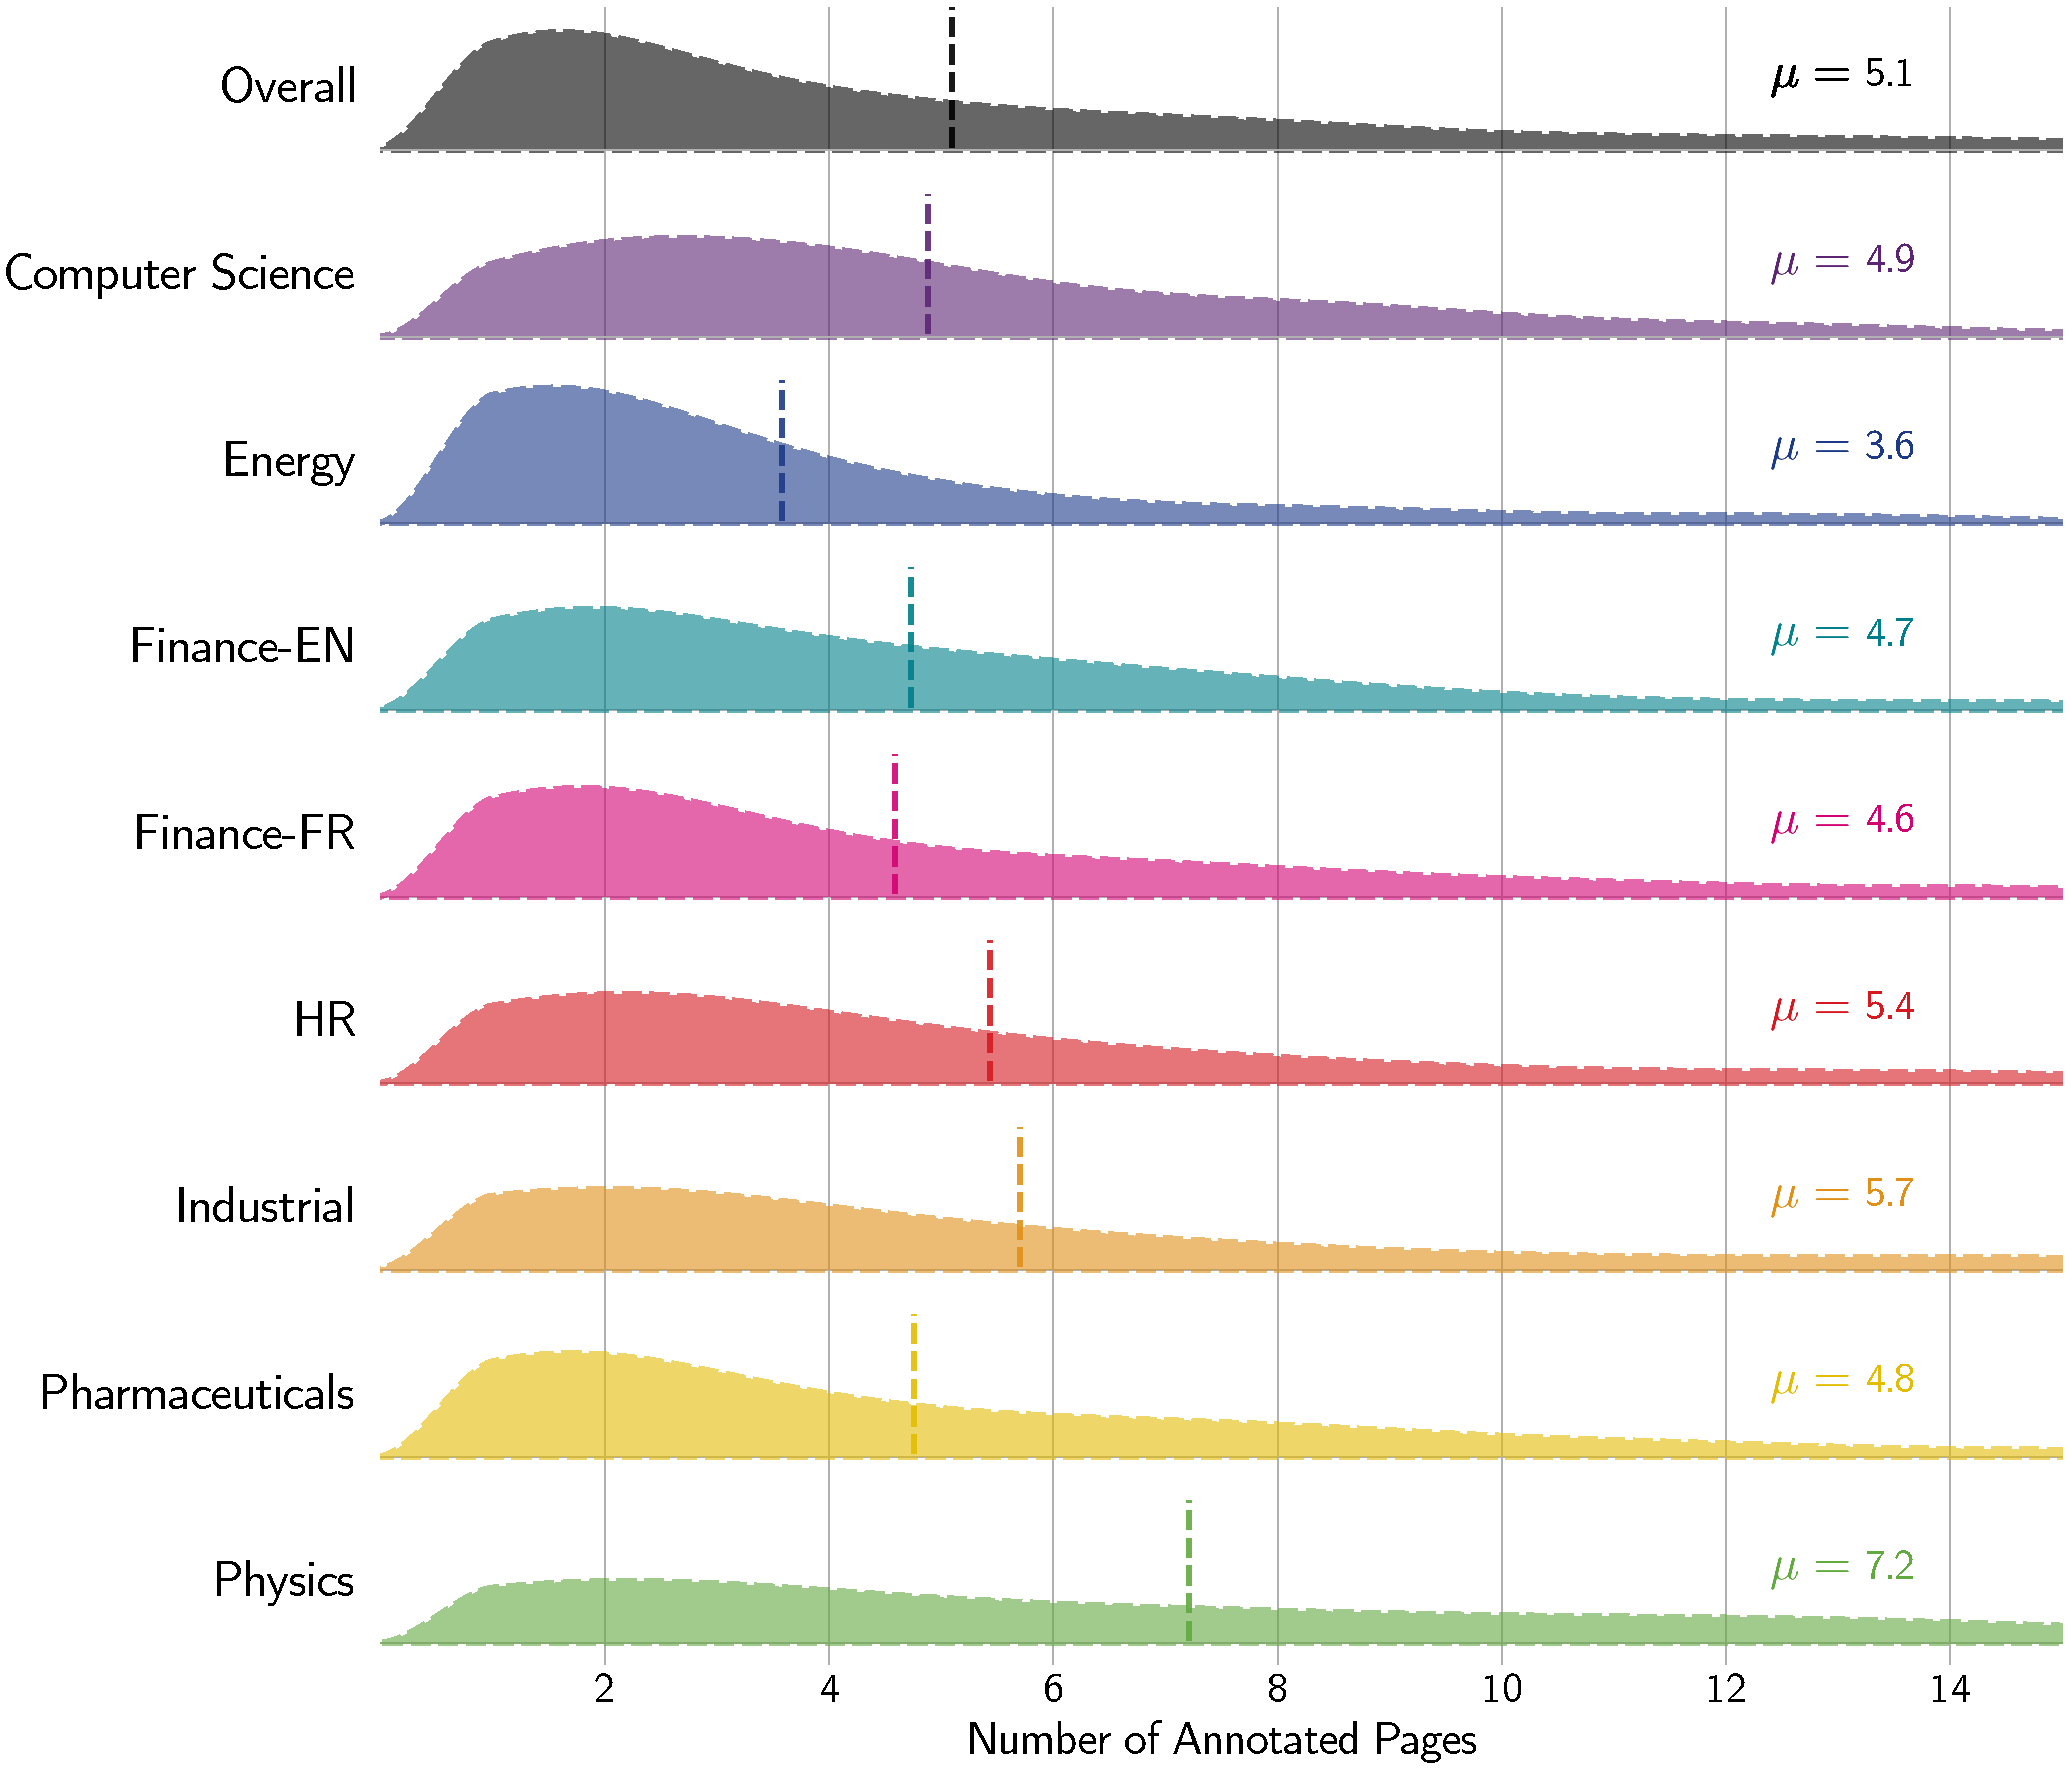
\includegraphics[clip, width=0.7\textwidth]{images/vidorev3_images/ridge_plot.pdf}
%     \caption{\textbf{Distribution of annotated page counts across domains.} This ridge plot displays the density of annotated pages per document for each specific domain, with vertical dashed lines marking the mean values. While the global average is $5.1$ pages, the distributions reveal distinct domain-specific characteristics: \textit{Physics} is a notable outlier, exhibiting the highest mean ($\mu=7.2$) and a heavy tail, suggesting that relevant information is often sparse and scattered across multiple pages. In contrast, \textit{Energy} queries appear more localized ($\mu=3.6$), with evidence typically concentrated within a narrower range.}
%     \label{fig:ridge_plot_query_types}
% \end{figure*}



\begin{figure*}[t!]
    \centering
    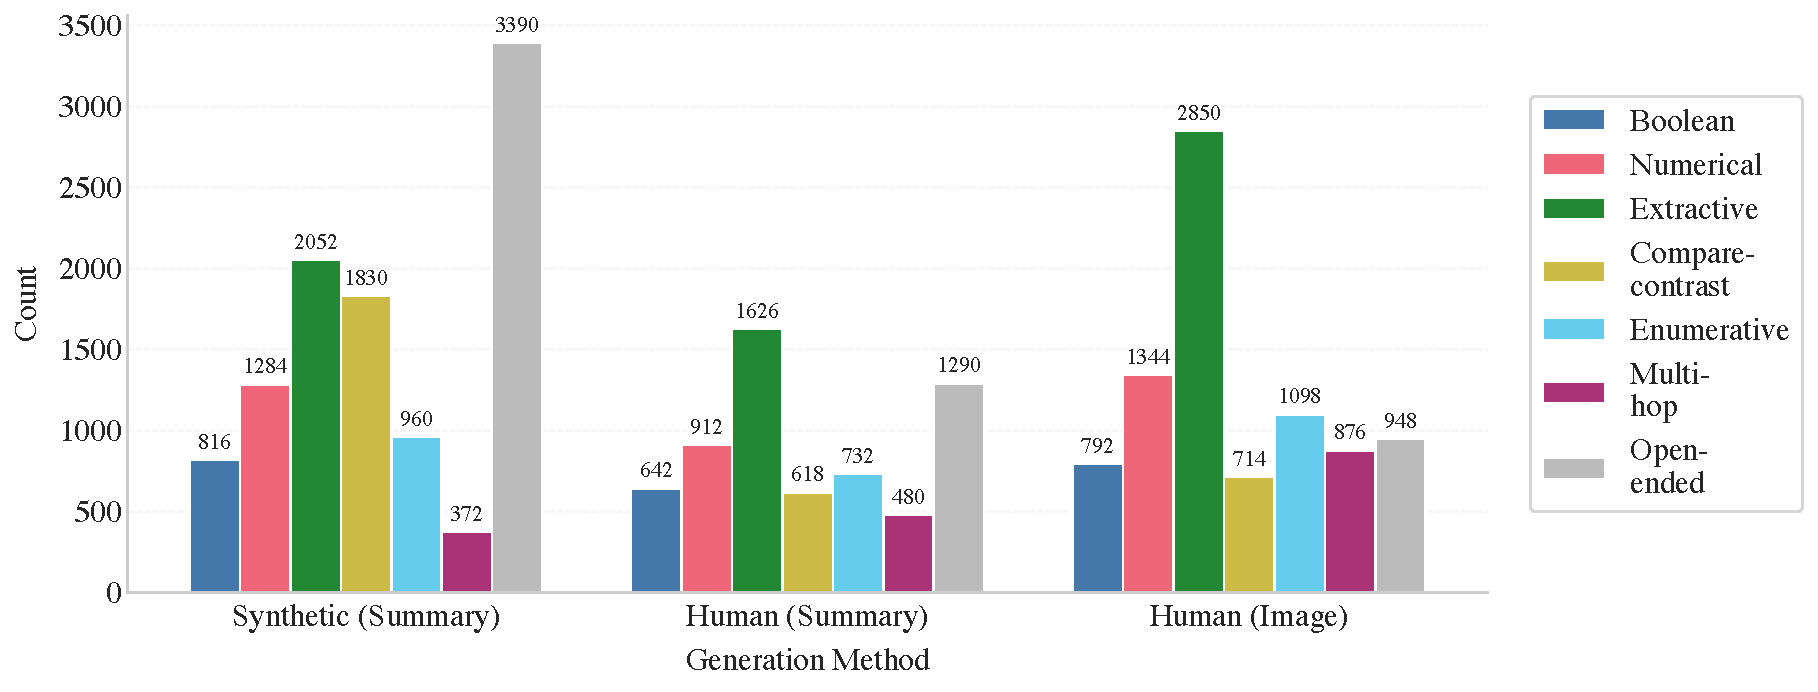
\includegraphics[clip, width=\textwidth]{images/vidorev3_images/query_types_by_generation_method.pdf}
    \caption{\textbf{Query type distribution by generation method.}}
    \label{fig:query type by generation method}
\end{figure*}

% \clearpage
% \paragraph{Page relevance scale}

% Table~\ref{tab:relevance_scale} details the relevance score rubrics provided to human annotator. Pages given a score of 0 were dropped from the final benchmark.

% \begin{table}[h]
% \small
% \centering
% \begin{tabular}{cXX}
% \toprule
% \textbf{Score} & \textbf{Label} & \textbf{Definition} \\
% \midrule
% 2 & Fully Relevant & The page contains the complete answer \\
% 1 & Critically Relevant & The page contains facts or information required to answer the query, though additional information is required \\
% 0 & Not Relevant & Provides no information relevant to the query \\
% \bottomrule
% \end{tabular}
% \caption{\textbf{Relevance scale used for page-level annotations.}}
% \label{tab:relevance_scale}
% \end{table}



%\paragraph{Ethics approval} 
%The annotation protocol was reviewed and approved by an ethics committee prior to the commencement of data collection. The review encompassed annotator recruitment procedures, compensation practices, task design, and data governance policies. Specific attention was given to ensuring that pay exceeded local minimum wage standards and that annotators were not exposed to harmful content. %\anto{Made up paragraph, we have to check with NVIDIA}


\begin{table}[H]
\centering

\resizebox{\columnwidth}{!}{%
\begin{tabular}{lccc}
\toprule
\textbf{Dataset} & \textbf{$\alpha$ (ord)} & \textbf{Gwet's AC2} \\ %& \textbf{Wgt. Agree} \\
\midrule
Computer science& 0.467 & 0.809 \\%& 0.849 \\
Energy & 0.463 & 0.714 \\%& 0.805 \\
Finance (EN) & 0.514 & 0.798 \\%& 0.832 \\
Finance (FR) & 0.320 & 0.736 \\%& 0.801 \\
H.R. & 0.413 & 0.793 \\%& 0.840 \\
Industrial Maintenance & 0.496 & 0.740 \\%& 0.803 \\
Telecom & 0.464 & 0.772 \\%& 0.833 \\
Nuclear & 0.389 & 0.794 \\%& 0.837 \\
Pharma & 0.478 & 0.755 \\%& 0.831 \\
Physics & 0.213 & 0.334 \\%& 0.668 \\
\midrule
\textbf{Overall} & \textbf{0.469} & \textbf{0.760} \\%& \textbf{0.815} \\
\bottomrule
\end{tabular}
}
\caption{Inter-annotator agreement for relevance ratings by dataset.}
\label{tab:iaa}
\end{table}



\begin{table*}[ht]
% \small
\centering
\begin{tabular}{lll}
\toprule
\textbf{Model alias} & \textbf{Full model name} & \textbf{Reference} \\ \midrule
Qwen3-8B & Qwen3-Embedding-8B & \cite{qwen3embedding} \\
Jina-v4 & jina-embeddings-v4 & \cite{günther2025jinaembeddingsv4universalembeddingsmultimodal} \\
Qwen3-0.6B & Qwen3-Embedding-0.6B & \cite{qwen3embedding} \\
LFM2-350M & LFM2-ColBERT-350M & \cite{liquidai2025lfm2} \\
BGE-M3 & BGE-M3 & \cite{chen_bge_2024} \\
BM25S & BM25S & \cite{bm25s} \\
ColEmbed-3B-v2 & llama-nemoretriever-colembed-3b-v2 & \cite{xu2025llamanemoretrievercolembedtopperforming} \\ % asked Gabriel about this
ColNomic-7B & colnomic-embed-multimodal-7b & \cite{nomicembedmultimodal2025} \\
ColEmbed-3B & llama-nemoretriever-colembed-3b-v1 & \cite{xu2025llamanemoretrievercolembedtopperforming} \\
ColNomic-3B & colnomic-embed-multimodal-3b & \cite{nomicembedmultimodal2025} \\
ColEmbed-1B & llama-nemoretriever-colembed-1b-v1 & \cite{xu2025llamanemoretrievercolembedtopperforming} \\
ColQwen2.5 & colqwen2.5-v0.2 & \cite{faysse2025colpaliefficientdocumentretrieval} \\
Nomic-7B & nomic-embed-multimodal-7b & \cite{nomicembedmultimodal2025} \\
ColQwen2 & colqwen2-v1.0 & \cite{faysse2025colpaliefficientdocumentretrieval} \\
Nomic-3B & nomic-embed-multimodal-7b & \cite{nomicembedmultimodal2025} \\
ColPali & colpali-v1.3 & \cite{faysse2025colpaliefficientdocumentretrieval} \\
Mxbai Edge 32M & mxbai-edge-colbert-v0-32m & \cite{takehi2025fantasticsmallretrieverstrain} \\
GTE-ModernColBERT & GTE-ModernColBERT-v1 & \cite{GTE-ModernColBERT} \\
ColModernVBERT & colmodernvbert & \cite{teiletche2025modernvbert} \\
ColSmol-256M & colSmol-256M & \cite{marafioti2025smolvlmredefiningsmallefficient} \\
\bottomrule
\end{tabular}
\caption{\textbf{Retriever reference table.} Model aliases used in Tables~\ref{tab:retriever_comparison_updated},~\ref{tab: english-only retrieval}, and~\ref{tab: french-only retrieval} are mapped to their HuggingFace model name and citation.}
\label{tab:model_metadata}
\end{table*}

% \paragraph{Retrieval performance with model size}

% \vic{To fill}

% \begin{figure}[h!]
%     \centering
%     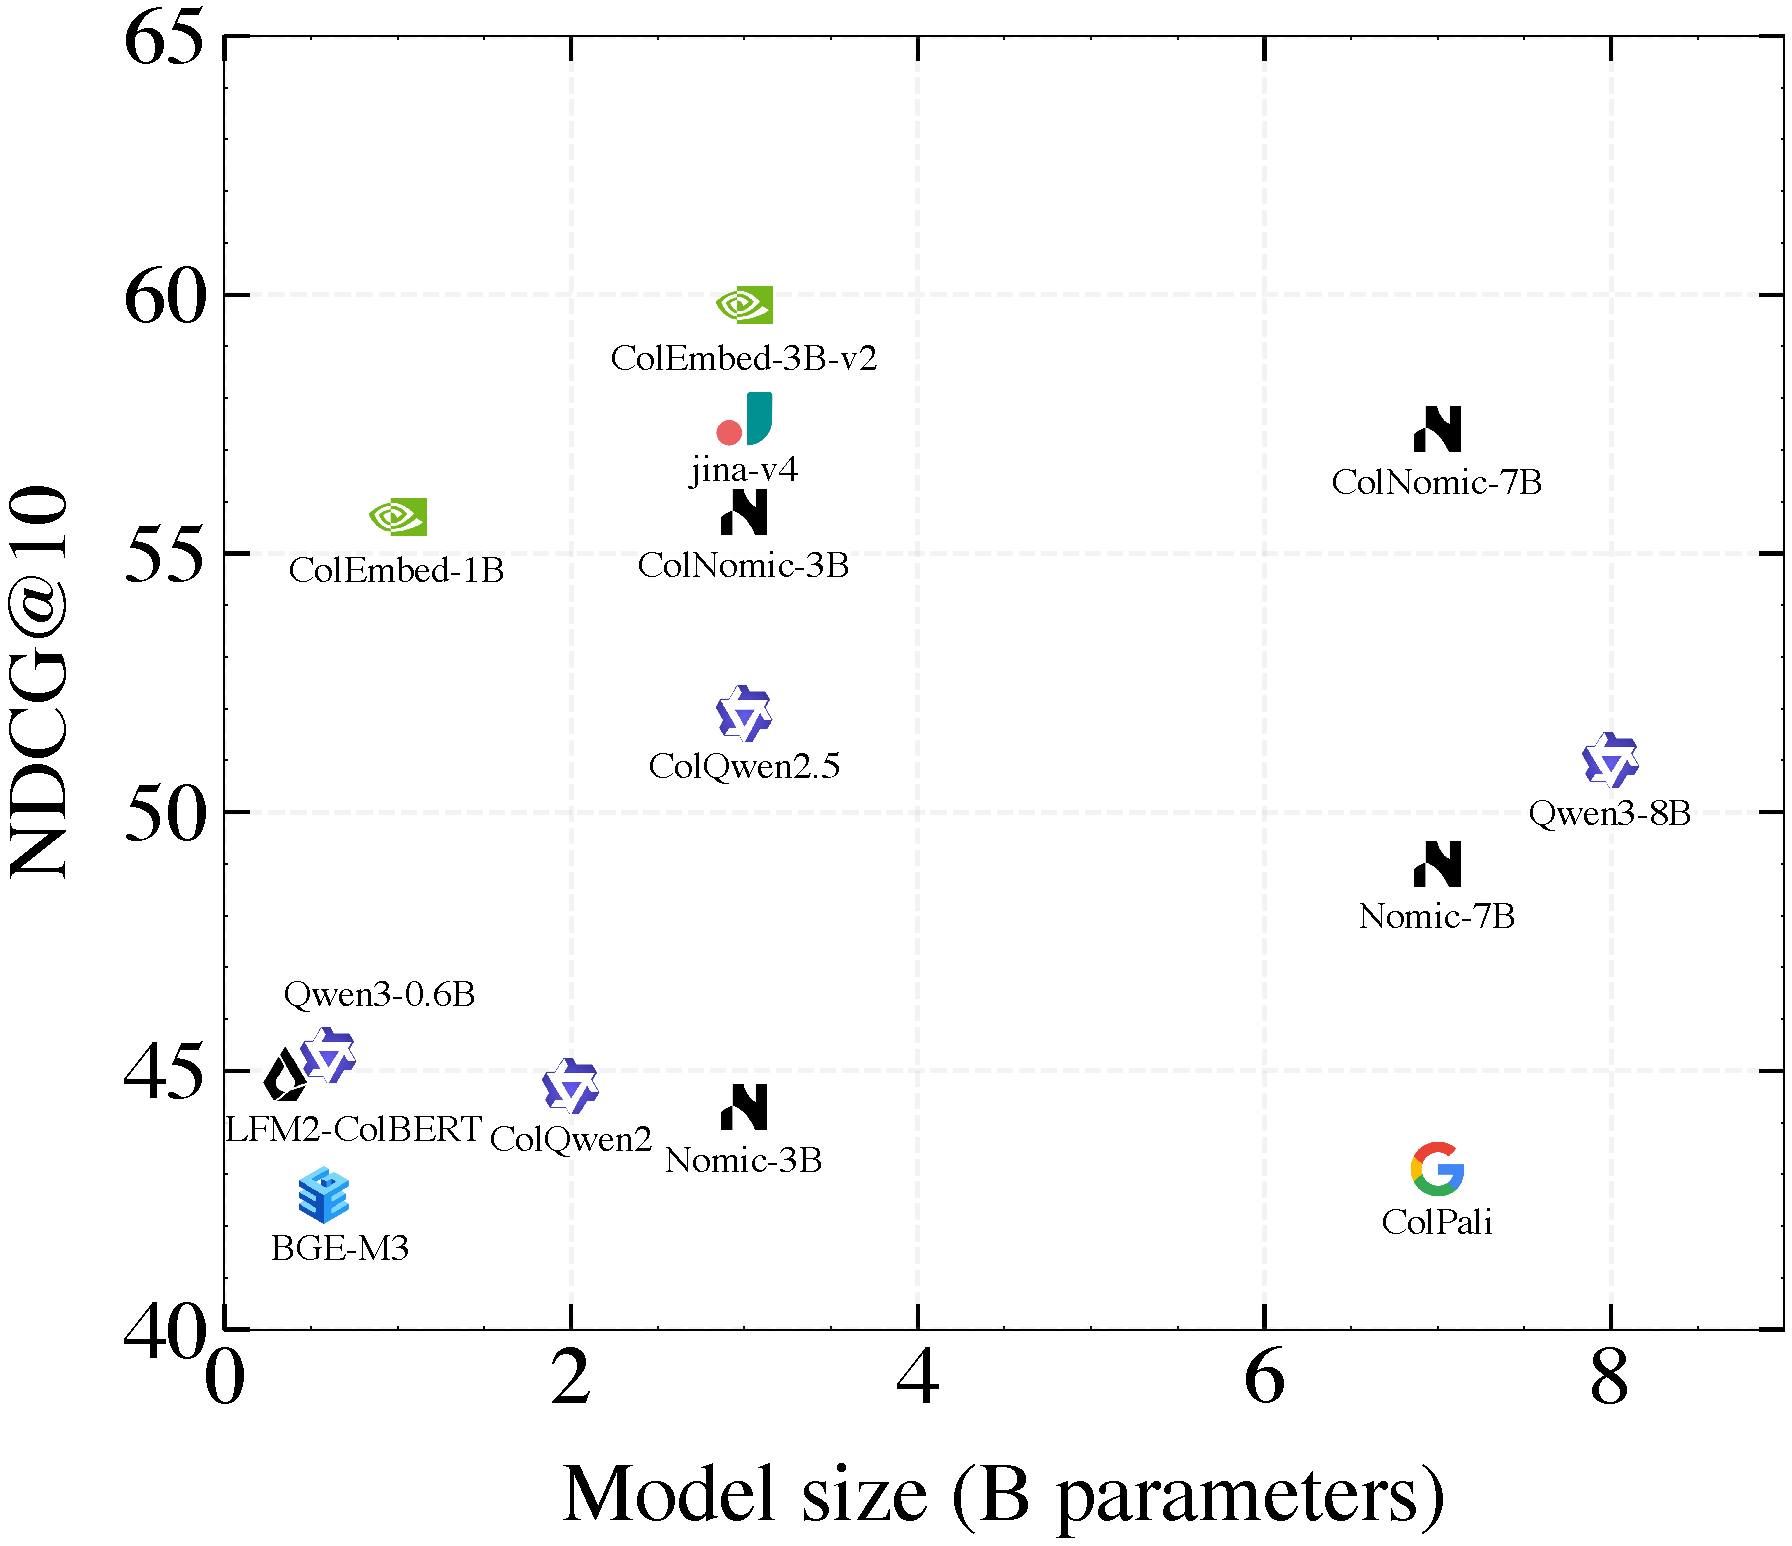
\includegraphics[width=\columnwidth]{images/vidorev3_images/size-performance_large_no_tomoro.pdf}
%     \caption{\textbf{Scaling of benchmark retrieval performance with model size.}} 
%     \label{fig:size-performance}
% \end{figure}


\begin{table*}[h!]
\centering
%\resizebox{\textwidth}{!}{%
\begin{tabular}{l c c c c c c c c >{\columncolor{avgcol}}c}
\toprule
\textbf{Model} & Size (B) & C.S. & Nucl. & Fin. & Phar. & H.R. & Ind. & Tele. & \textbf{Average} \\
\midrule
\multicolumn{9}{l}{\textit{\textbf{Textual Retrievers}}} \\
Jina-v4	& 3 & 67.3	& \textbf{48.2} & \textbf{56.5}&  59.0& \textbf{58.8} & 	45.8	& 61.0	& \textbf{56.7}\\
Qwen3-8B$^\bigstar$	& 8 & \textbf{73.5}	& 42.2	 & 54.8	& 62.4	& 52.3	& 45.3	& \textbf{66.0}	& 56.6 \\
LFM2-350M & 0.35 & 70.6 & 45.4 & 48.3 & 62.1 & 53.2 & \textbf{47.9} & 63.8 & 55.9\\
Mxbai Edge 32M & 0.03 & 68.0 & 44.4 & 48.2 & \textbf{62.5} & 52.7 & 47.1 & 61.9 & 55.0 \\
BM25S	& - & 64.7&	45.9&	49.9&	56.9&	49.6&	45.6	&58.3	&53.0\\
Qwen3-0.6B$^\bigstar$& 0.6 &	70.5	& 39.7	&51.5	& 57.4	& 46.2	&42.4	&59.7	&52.3\\
GTE-ModernColBERT & 0.15 & 63.6 & 41.7 & 39.8 & 62.0 & 46.2 & 44.6 & 59.7 & 51.1\\
BGE-M3$^\bigstar$	& 0.57 &63.6&	34.3	& 43.9	&54.7	&45.3	&39.0	&54.3	&47.9\\
\midrule
\multicolumn{9}{l}{\textit{\textbf{Visual Retrievers}}} \\
% tomoro-colqwen3-8b$^\blacktriangle$ & 77.6 & \textbf{53.7} & \textbf{70.8} & \textbf{68.1} & \textbf{66.8} & \textbf{58.9} & 70.8 & \textbf{66.7}\\
% tomoro-colqwen3-4b$^\blacktriangle$ & 78.0 & 52.3 & 69.7 & 67.8 & 64.1 & 58.8 & \textbf{72.5} & 66.2\\
ColEmbed-3B-v2 & 3 & \textbf{78.6} & 52.9 & 69.1 & \textbf{67.6} & \textbf{65.4} & 56.8 & \textbf{71.7} & \textbf{66.0} \\
ColEmbed-3B & 3 & 77.8 & \textbf{53.4} & \textbf{69.5 }& 66.9 & 64.9 & \textbf{57.0} & 69.4 & 65.6 \\
ColEmbed-1B & 1 & 75.5 & 52.2 & 67.0 & 66.2 & 64.5 & 56.1 & 68.7 & 64.3 \\
Jina-v4 & 3 & 74.2 & 52.4 & 66.1 & 65.2 & 64.6 & 55.9 & 68.7 & 63.9 \\
ColNomic-7B & 7 & 78.2 & 48.2 & 63.1 & 64.6 & 62.9 & 54.2 & 69.6 & 63.0 \\
ColNomic-3B & 3 & 75.5 & 45.5 & 63.0 & 63.7 & 62.6 & 52.8 & 68.6 & 61.7 \\
ColQwen2.5 & 3 & 75.2 & 42.9 & 61.2 & 60.9 & 59.2 & 49.4 & 65.3 & 59.2 \\
Nomic-7B$^\bigstar$ & 7 & 70.9 & 42.3 & 57.6 & 63.8 & 55.9 & 48.5 & 62.0 & 57.3 \\
ColQwen2 & 2 & 73.5 & 44.1 & 50.9 & 58.1 & 54.7 & 49.8 & 63.2 & 56.3 \\
ColPali & 7 & 72.5 & 38.1 & 43.3 & 57.7 & 53.3 & 47.0 & 59.2 & 53.0 \\
Nomic-3B$^\bigstar$ & 3 & 62.1 & 37.2 & 53.3 & 59.2 & 51.9 & 41.1 & 57.2 & 51.7 \\
ColModernVBERT & 0.25 & 59.7 & 42.0 & 50.4 & 56.6 & 47.0 & 43.9 & 55.2 & 50.7 \\
ColSmol-256M & 0.25 & 57.4 & 36.5 & 47.7 & 51.4 & 46.0 & 38.5 & 47.5 & 46.4 \\
\bottomrule
\end{tabular}
%}
\caption{\textbf{English-only retrieval performance (NDCG@10).} $\bigstar$: single-vector models. Results are computed on the English queries of the English datasets.}
\label{tab: english-only retrieval}
\end{table*}


\begin{table*}[h!]
\small
\centering
%\resizebox{\textwidth}{!}{%
\begin{tabular}{l c c c c >{\columncolor{avgcol}}c}
\toprule
\textbf{Model} & Size (B) & Phys. & Ener. & Fin. & \textbf{Average} \\
\midrule
\multicolumn{5}{l}{\textit{\textbf{Textual Retrievers}}} \\
Jina-v4	& 3 & 44.0	& \textbf{63.4}	& \textbf{44.8} & \textbf{50.7}\\
Qwen3-8B$^\bigstar$	& 8 &\textbf{45.8}	& 60.2	& 37.6& 47.9\\
Qwen3-0.6B$^\bigstar$	& 0.6 & 43.8	& 54.9	& 28.5& 42.4\\
BGE-M3$^\bigstar$ &0.57	& 38.3	& 53.1	& 28.4&39.9\\
BM25S	& - & 39.8	& 57.4	& 35.9 & 44.4\\
\midrule
\multicolumn{5}{l}{\textit{\textbf{Visual Retrievers}}} \\
ColEmbed-3B-v2 & 3 & 48.2 & 67.5 & 48.2 & \textbf{54.6}\\
ColNomic-7b	& 7 & \textbf{48.5} & 67.0	& 47.9 & 54.5\\
ColNomic-3b	& 3 & \textbf{48.5} &	\textbf{67.9} &	46.8 & 54.4\\
Jina-v4	& 3 & 46.8	& 66.7 & 48.6 & 54.0 \\
ColEmbed-3B & 	3 & 46.6 &	66.3 &	\textbf{48.9} & 53.9\\
ColEmbed-1B & 1 & 44.7 &	64.6 &	47.8 & 52.4\\
ColQwen2.5 &	3 & 47.8	&62.3	&43.6& 51.2\\
Nomic-7B$^\bigstar$ &	7 & 45.6&	61.6&	41.3 & 49.5\\
ColQwen2	& 3 & 43.9	&55.6	&26.5& 42.0\\
Nomic-3B$^\bigstar$	& 3 & 43.6	&56.4	&34.4 & 44.8\\
ColPali	& 7 & 43.2	&50.5	&23.6 & 39.1 \\
%ColModernVBERT	&27.9&	44.2&	27.0 & 33.0 \\
%ColSmol-256M	&19.1	&31.9	&20.8 & 23.9 \\
\bottomrule
\end{tabular}
%}
\caption{\textbf{French-only retrieval performance (NDCG@10).} $\bigstar$: single-vector models. Results are computed on the French queries of the French datasets.}
\label{tab: french-only retrieval}
\end{table*}

% \clearpage

\paragraph{Additional Retrieval Modality Performances} To evaluate the hybrid retrieval setup, we use the multimodal Jina-v4 model to generate separate visual and textual rankings. We then construct a hybrid retrieval set by merging the top-5 results from each modality and removing duplicates. Because this set-union operation does not preserve a strict ranking order, we report the unranked F1 score. As shown in \Cref{tab:hybrid_comparison}, the hybrid approach consistently outperforms single-modality baselines.

% \clearpage


\begin{table*}[t!]
\centering
% \resizebox{\columnwidth}{!}{%
\small
\begin{tabular}{l c c c c c c c c c c >{\columncolor{avgcol}}c}
\toprule
 & \multicolumn{7}{c}{\textbf{English Datasets}} & \multicolumn{3}{c}{\textbf{French Datasets}} & \multicolumn{1}{c}{} \\
\cmidrule(lr){2-8} \cmidrule(lr){9-11}
\textbf{Modality} & \shortstack{C.S.} & \shortstack{Nucl.} & \shortstack{Fin.} & \shortstack{Phar.} & \shortstack{H.R.} & \shortstack{Ind.} & \shortstack{Tel.} & \shortstack{Phys.} & \shortstack{Ener.} & \shortstack{Fin.} & \textbf{Avg.} \\
\midrule
Visual	& 39.4	& 25.5	& 28.4	& 27.5	& 30.0	& 21.4	& 31.4	&\textbf{26.6}	& 25.2	& 22.9	& 27.8 \\
Textual	& 35.4	& 23.1&	24.5	&24.2	&27.4&	16.5&	29.0&	25.8 &	23.9	&20.4&	25.0 \\
Hybrid	&\textbf{43.0}	&\textbf{27.7}	&\textbf{30.9}	&\textbf{29.7}	&\textbf{32.6}	&\textbf{22.2}	&\textbf{35.5}&	26.5	&\textbf{29.8}	&\textbf{24.3}	&\textbf{30.2} \\
\midrule
\textit{Avg. \# Pages for hybrid}	&\textit{6.96}	& \textit{7.38}	&\textit{7.77}&\textit{7.40}&	\textit{7.29}&	\textit{7.77}	&\textit{7.09} &	\textit{7.26}&	\textit{6.97}	&\textit{7.61}&	\textit{7.35} \\
\bottomrule
\end{tabular}
% }
\caption{\textbf{Performance comparison of retrieval modalities (F1@10) on Jina-v4.} Evaluation is performed using the multimodal retriever Jina-v4. The Hybrid method combines the top-5 visual and top-5 textual matches, subsequently removing duplicates. The final row reports the average number of unique pages remaining in the hybrid set. The Hybrid setup constantly outperforms both textual and visual retrieval.}
\label{tab:hybrid_comparison}
\end{table*}


% \clearpage

% \newpage


\section{ColEmbed-3B-v2 performance breakdown}\label{appendix: colembed-v2-perf-breakdown}

\Cref{tab:perf language} details the retrieval scores of ColEmbed-3B-v2 by query language, highlighting small performance variations by language.

% \begin{table}[h!]
% \centering
% \resizebox{\columnwidth}{!}{%
% \begin{tabular}{l ccc c}
% \toprule
% & \multicolumn{3}{c}{\textbf{Query Format}} & \\ % Labels the columns
% \cmidrule(lr){2-4}
% \textbf{Query Type} & Instruction & Keyword & Question & \textbf{Avg.} \\
% \midrule
% Boolean & — & — & 70.3 & 70.3 \\
% Numerical & 65.0 & 64.9 & 67.6 & 66.3 \\
% Extractive & 63.3 & 65.6 & 67.3 & 65.8 \\
% Compare-contrast & 59.3 & 59.2 & 61.3 & 60.0 \\
% Enumerative & 56.2 & 65.2 & 57.8 & 57.6 \\
% Multi-hop & 50.6 & — & 57.1 & 53.9 \\
% Open-ended & 48.0 & 45.8 & 50.6 & 48.6 \\
% \midrule
% \textbf{Avg.} & 55.6 & 56.4 & 62.6 & 59.5 \\
% \bottomrule
% \end{tabular}
% }
% \caption{\textbf{ColEmbed-3B-v2 NDCG@10 by query type and format.}}
% \label{tab:perf query type format}
% \end{table}

\paragraph{Performance by number of annotated pages}

As seen in Figure~\ref{fig:perf number of pages}, performance drops with the number of annotated pages. However, a potential confounding factor is the correlation between query type and the number of annotated pages, since more complex query types also have higher number of annotated pages (Figure~\ref{fig:num pages per query type}). We perform a stratified regression analysis to isolate these two effects.



We model NDCG@10 as a linear function of the number of annotated pages ($P$) stratified by query type. For each of the 7 query types, we fit an ordinary least squares regression:
\begin{equation*}
    NDCG@10 = a \cdot P + b + \epsilon.
\end{equation*}

Results in Figure~\ref{fig:perf content num pages} and Table~\ref{tab:num pages content type decay} reveal that all query types suffer a significant performance penalty as the number of annotated pages increases. Slope values are nearly uniform ($a \approx -0.024$), suggesting a similar drop in retrieval accuracy across most query types. The open-ended and enumerative types are the two exceptions: despite having the lowest NDCG@10 for low page counts, they also have the shallowest slope, which suggests that retrieval success on these queries is constrained by the model's fundamental difficulty in synthesizing multiple relevant sources rather than the volume of relevant context.

\begin{table}[!h]
\small
\centering
%\resizebox{\columnwidth}{!}{%
\begin{tabular}{lc}
\toprule
\textbf{Query Language} & \textbf{NDCG@10}\\
\midrule
English & 60.8 \\
French & 59.8 \\
Portuguese & 59.6 \\
Spanish & 59.6 \\
Italian & 59.1 \\
German & 57.9 \\
\bottomrule
\end{tabular}
%}
\caption{\textbf{ColEmbed-3B-v2 NDCG@10 by query language.}}
\label{tab:perf language}
\end{table}

\begin{figure}[t]
    \centering
    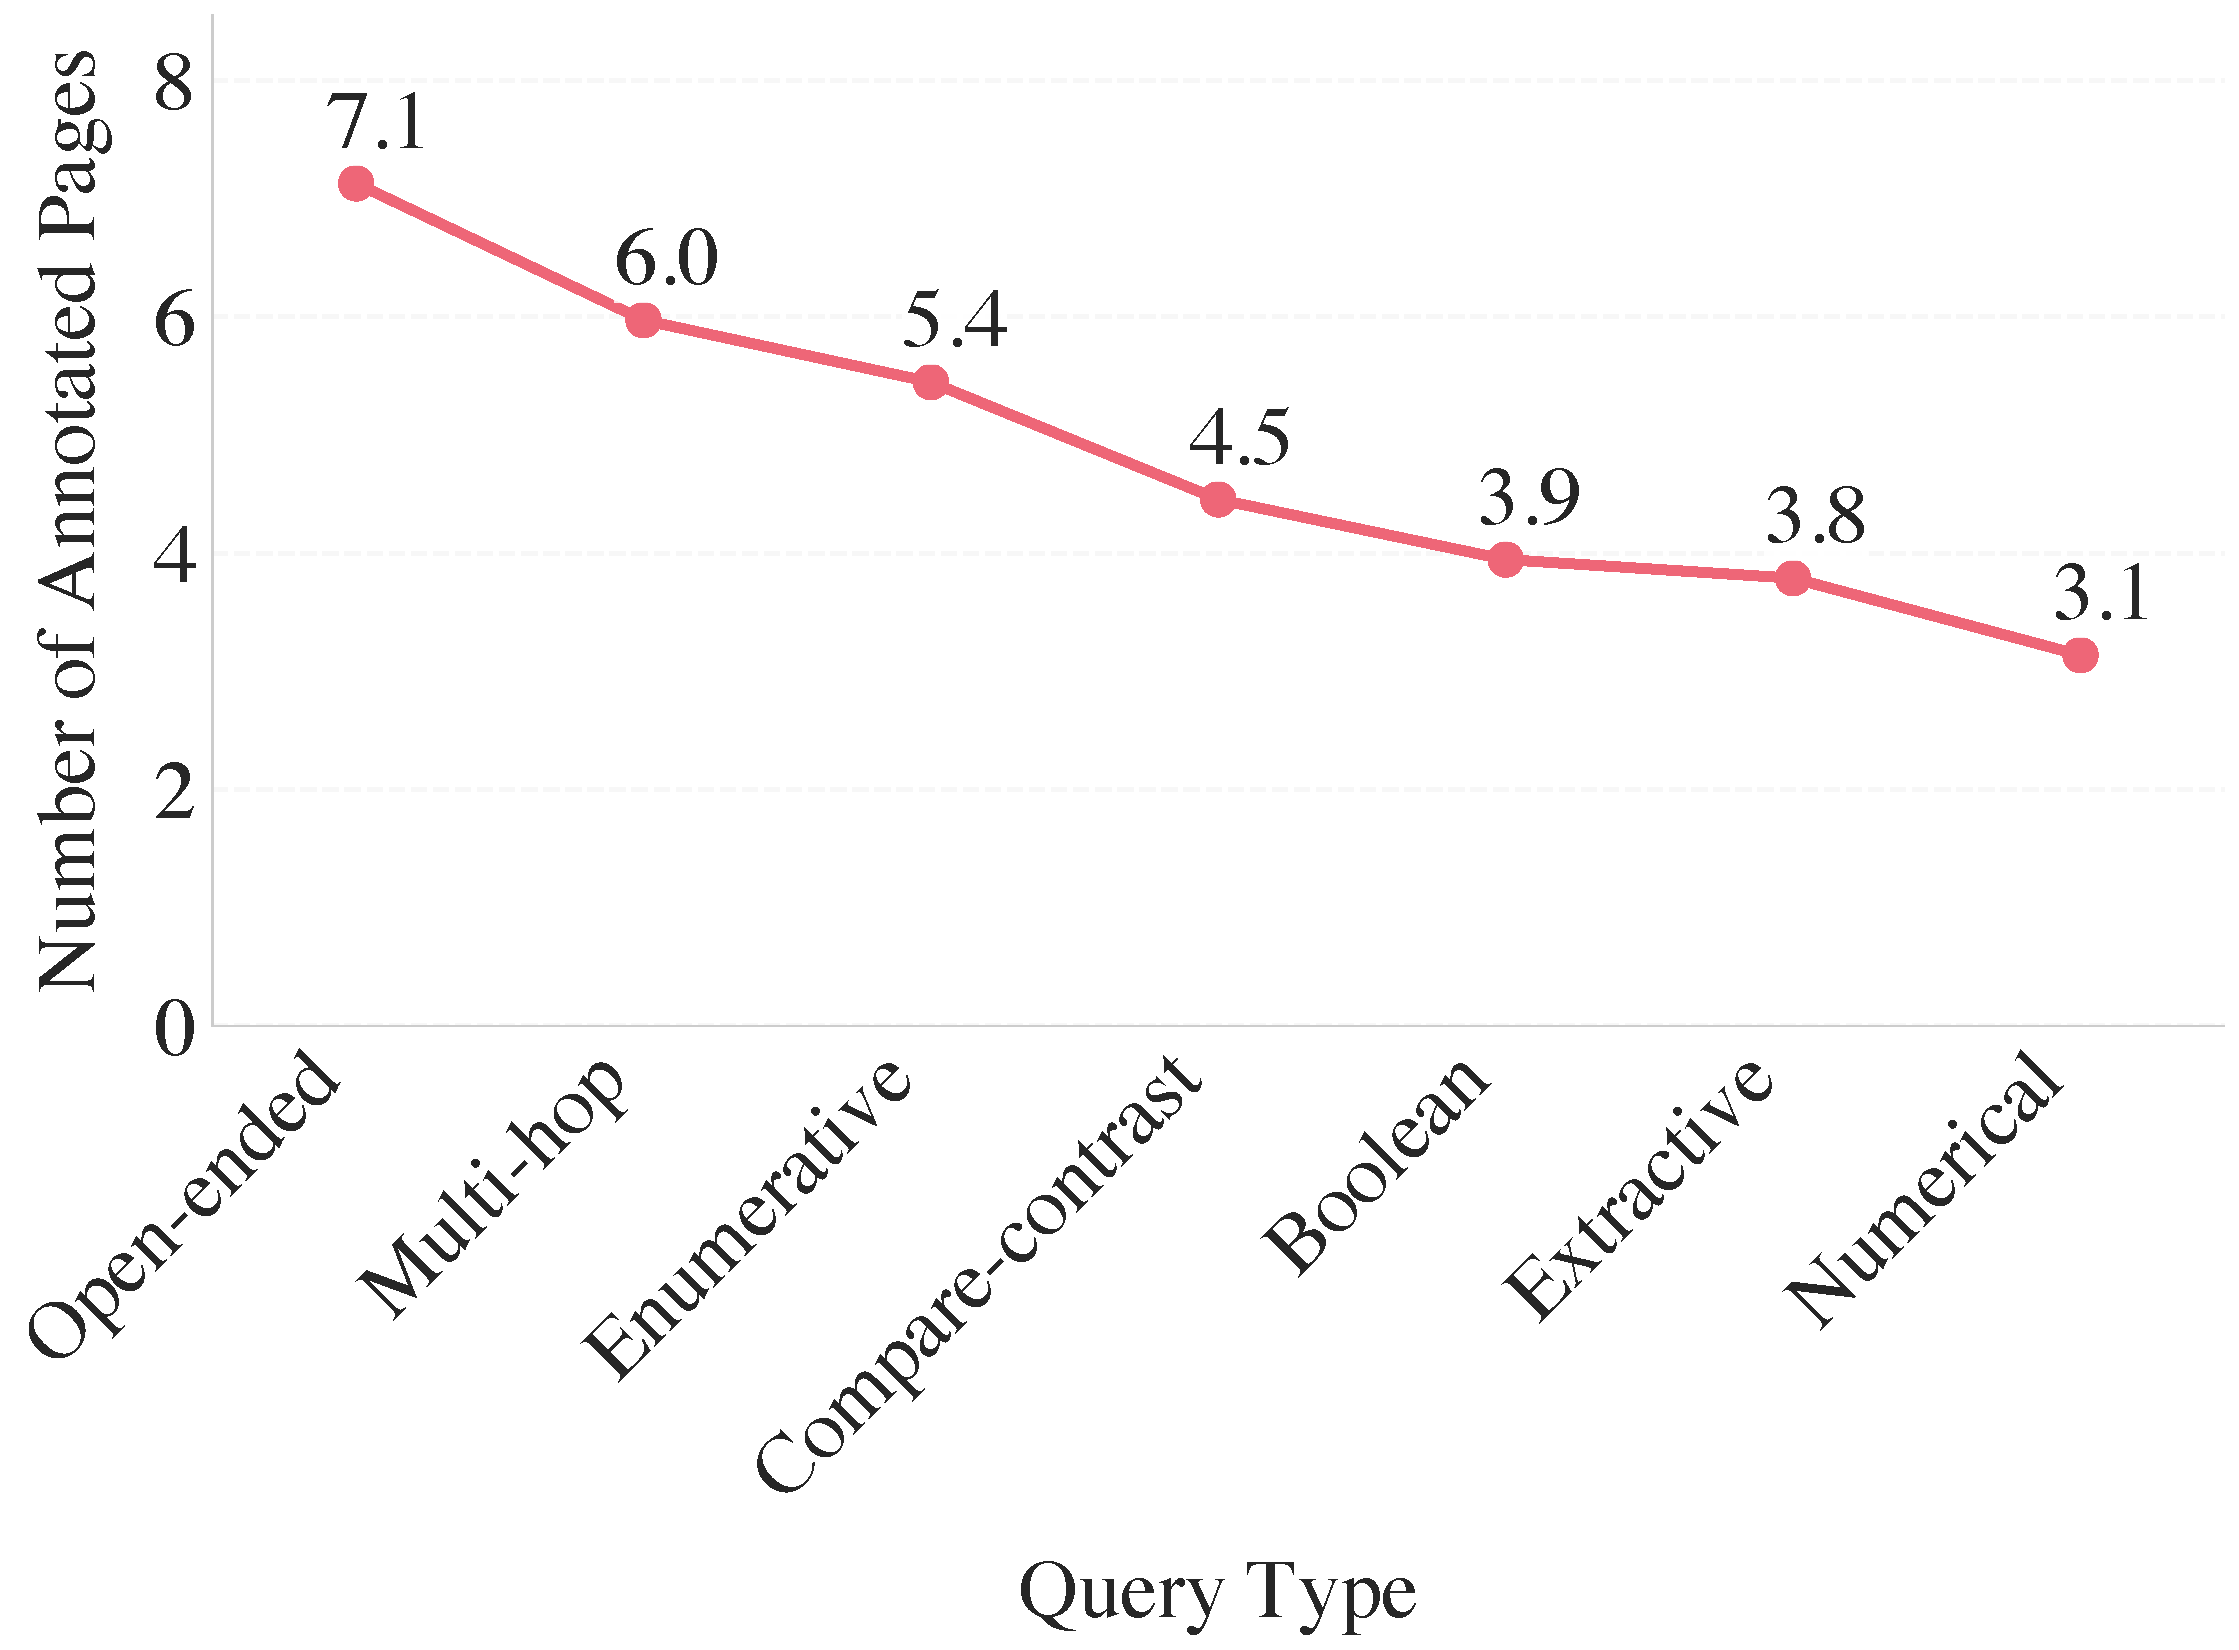
\includegraphics[width=0.9\columnwidth]{images/vidorev3_images/annotated_pages_by_query_type.pdf}
    \caption{\textbf{Average number of annotated pages by query type.}} 
    \label{fig:num pages per query type}
\end{figure}

\begin{figure}[h!]
    \centering
    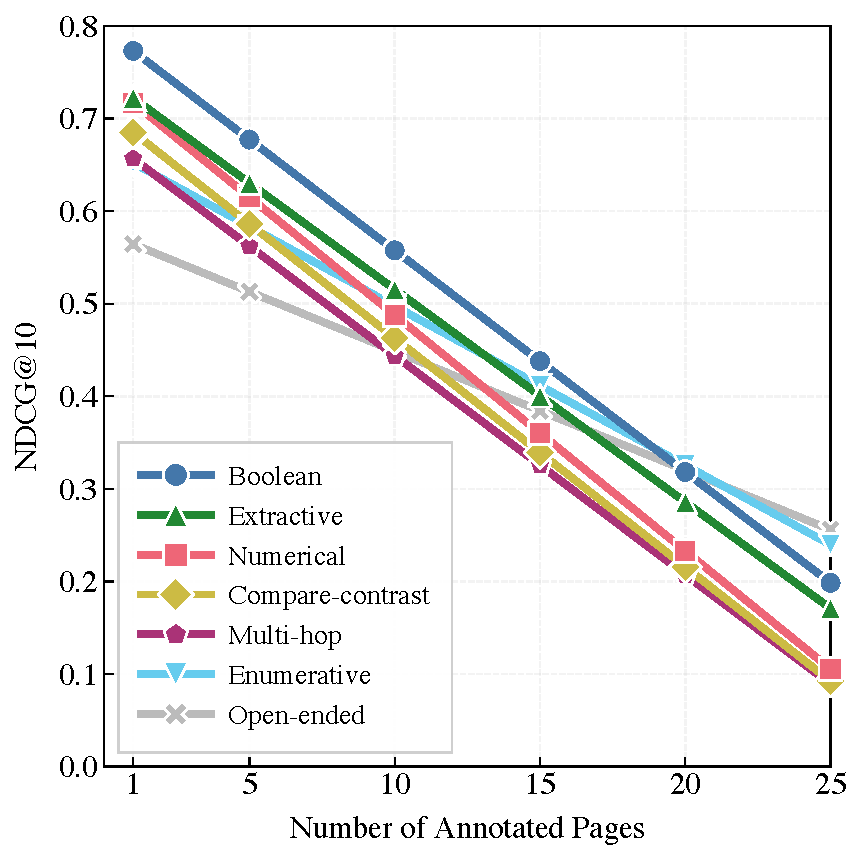
\includegraphics[width=0.8\columnwidth]{images/vidorev3_images/ndcg_query_type_num_pages.pdf}
    \caption{\textbf{ColEmbed-3B-v2 NDCG@10 by number of annotated pages and query type.}} 
    \label{fig:perf content num pages}
\end{figure}

\begin{table}[h!]
\centering
\small
\begin{tabular}{lccc}
\toprule
\textbf{Query Type} & Slope $a$ & Intercept $b$ & $R^2$ \\
\midrule
Boolean           & -0.0239 & 0.797 & 0.101 \\
Numerical         & -0.0255 & 0.742 & 0.059 \\
Extractive        & -0.0230 & 0.745 & 0.084 \\
Compare-contrast  & -0.0247 & 0.710 & 0.117 \\
Enumerative       & -0.0172 & 0.669 & 0.080 \\
Multi-hop         & -0.0237 & 0.680 & 0.114 \\
Open-ended        & -0.0129 & 0.577 & 0.057 \\
\bottomrule
\end{tabular}
\caption{\textbf{Linear regression analysis of NDCG@10 decay with number of annotated pages, by query type.} The slope $a$ represents performance sensitivity to retrieval context size, while the intercept $b$ represents intrinsic difficulty at minimum context size.}
\label{tab:num pages content type decay}
\end{table}

\paragraph{Performance by content type}

NDCG@10 by content type in Table~\ref{tab:perf content type} show that retrieval is more challenging for visual content, with Image performing 10pp below Text. However, content type and query type are correlated in our benchmark: for instance, tables appear in numerical queries 2.2 $\times$ more often than the baseline, while images are over-represented in open-ended queries (Figure~\ref{fig:lift content type}). Since numerical queries are easier than open-ended ones, we test whether the effect of content type is a byproduct of query type confounding. We fit an additive model that predicts performance as the sum of independent query-type and content-type effects. Figure~\ref{fig:ndcg content query residuals heatmap} shows the residuals which measure deviation from this baseline. We see that most residuals are below 5pp, indicating that the two factors combine additively without significant interaction.


\begin{table}[h!]
\small
\centering
%\resizebox{\columnwidth}{!}{%
\begin{tabular}{lcc}
\toprule
\textbf{Content type} & NDCG@10 & Content type count \\
\midrule
Text & 59.3 & 17244 \\
Chart & 56.3 & 2364 \\
Infographic & 55.2 & 2814 \\
Table & 53.9 & 6480 \\
Other & 50.8 & 492 \\
Image & 49.3 & 1140 \\
Mixed & 45.1 & 1164 \\
\bottomrule
\end{tabular}
%}
\caption{\textbf{ColEmbed-3B-v2 NDCG@10 by content type.} Content type is labeled on each annotated page based on the nature of the query-relevant content delimited by the bounding boxes. One page may be tagged with several content types if it contains multiple relevant sections of distinct nature. The Mixed type corresponds to annotations encompassing several content types.}
\label{tab:perf content type}
\end{table}

\begin{figure}[h!]
\centering
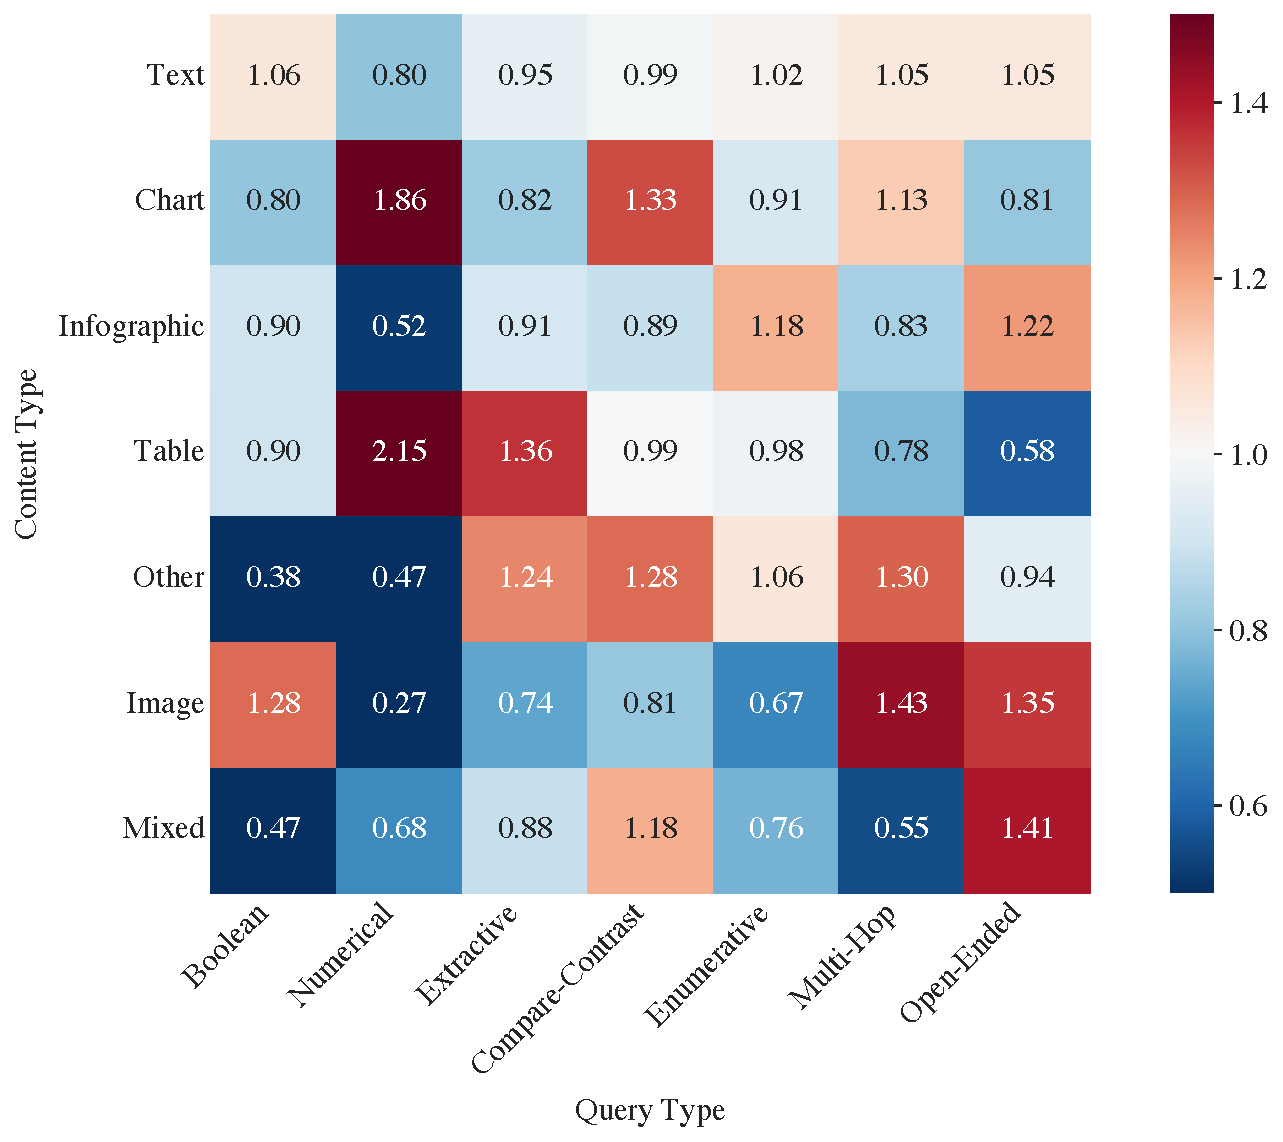
\includegraphics[width=\columnwidth]{images/vidorev3_images/lift_content_query_type.pdf}
\caption{\textbf{Lift of query types by content type.} Each cell shows the ratio of observed query type frequency to baseline frequency for a given content type. Values >1 indicate over-representation (e.g., tables appear 2.15× more in numerical queries than expected), while values <1 indicate under-representation.}
\label{fig:lift content type}
\end{figure}

\begin{figure}[h!]
\centering
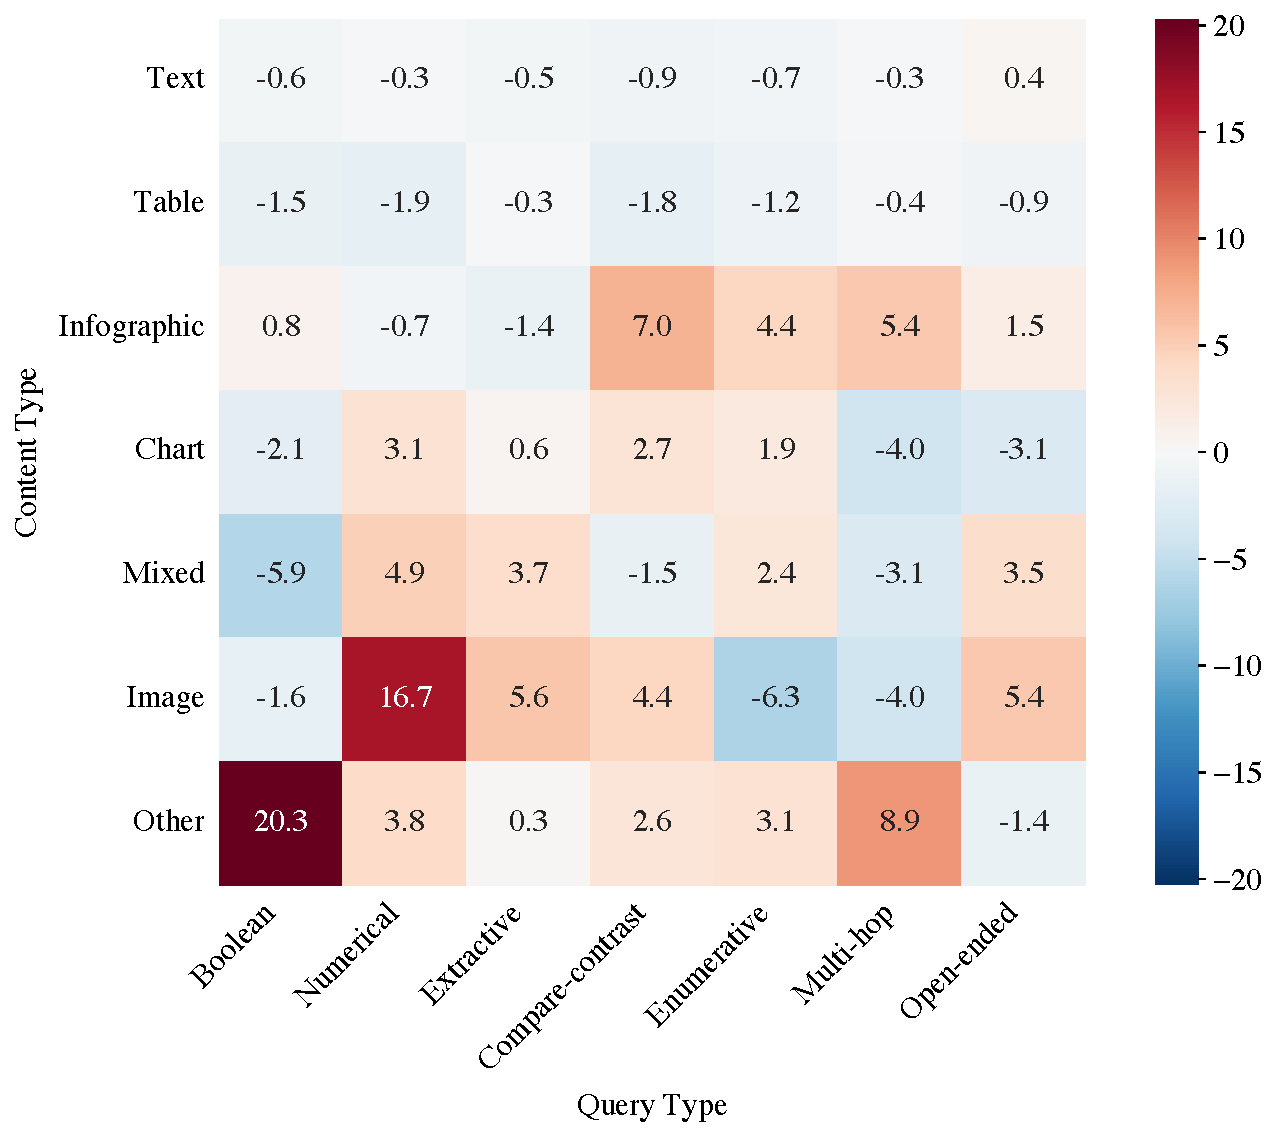
\includegraphics[width=\columnwidth]{images/vidorev3_images/ndcg_content_query_residuals_heatmap.pdf}
\caption{\textbf{Residuals from additive performance model.} Each cell shows the difference between observed NDCG@10 and the value predicted by an additive model of query type and content type main effects. Values near zero (white) indicate no interaction; positive values (red) indicate better-than-expected performance for that combination; negative values (blue) indicate worse-than-expected.} 
\label{fig:ndcg content query residuals heatmap}
\end{figure}

% \begin{table}[h!]
% \centering
% \resizebox{\columnwidth}{!}{%
% \begin{tabular}{lcc}
% \toprule
% Query format & NDCG@10 & Query count \\
% \midrule
% Question & 62.6 & 9936 \\
% Keyword & 56.4 & 2988 \\
% Instruction & 55.6 & 5670 \\
% \bottomrule
% \end{tabular}
% }
% \caption{\textbf{ColEmbed-3B-v2 NDCG@10 by query format.}}
% \label{tab:perf query format}
% \end{table}

% \begin{table}[h!]
% \centering
% \resizebox{\columnwidth}{!}{%
% \begin{tabular}{lcc}
% \toprule
% Query type & NDCG@10 & Query type count \\
% \midrule
% Boolean & 70.3 & 2250 \\
% Numerical & 66.3 & 3540 \\
% Extractive & 65.8 & 6528 \\
% Compare-contrast & 60.0 & 3162 \\
% Enumerative & 57.6 & 2790 \\
% Multi-hop & 53.9 & 1728 \\
% Open-ended & 48.6 & 5628 \\
% \bottomrule
% \end{tabular}
% }
% \caption{\textbf{colembed-3b-v2 NDCG@10 by query type.} The sum of the query type count column exceeds the number of individual queries since a query may have multiple tags,}
% \label{tab:perf query type}
% \end{table}

% \begin{table}[h!]
% \centering
% \resizebox{\columnwidth}{!}{%
% \begin{tabular}{l ccc c}
% \toprule
% & \multicolumn{3}{c}{\textbf{Query Format}} & \\ % Labels the columns
% \cmidrule(lr){2-4}
% \textbf{Query Type} & Instruction & Keyword & Question & \textbf{Mean} \\
% \midrule
% Boolean & — & — & 70.3 & 70.3 \\
% Numerical & 65.0 & 64.9 & 67.6 & 66.3 \\
% Extractive & 63.3 & 65.6 & 67.3 & 65.8 \\
% Compare-contrast & 59.3 & 59.2 & 61.3 & 60.0 \\
% Enumerative & 56.2 & 65.2 & 57.8 & 57.6 \\
% Multi-hop & 50.6 & — & 57.1 & 53.9 \\
% Open-ended & 48.0 & 45.8 & 50.6 & 48.6 \\
% \midrule
% \textbf{Mean} & 55.6 & 56.4 & 62.6 & 59.5 \\
% \bottomrule
% \end{tabular}
% }
% \caption{\textbf{colembed-3b-v2 NDCG@10 by query type and format.} The sum of the query type counts exceeds the number of individual queries since a query may have multiple tags.}
% \label{tab:perf query type format}
% \end{table}

% \begin{table}[h!]
% \centering
% \resizebox{\columnwidth}{!}{%
% \begin{tabular}{lcc}
% \toprule
% Content type & NDCG@10 & Content type count \\
% \midrule
% Text & 59.3 & 17244 \\
% Chart & 56.3 & 2364 \\
% Infographic & 55.2 & 2814 \\
% Table & 53.9 & 6480 \\
% Other & 50.8 & 492 \\
% Image & 49.3 & 1140 \\
% Mixed & 45.1 & 1164 \\
% \bottomrule
% \end{tabular}
% }
% \caption{\textbf{ColEmbed-3B-v2 NDCG@10 by content type.} Content type is labeled on each annotated page based on the nature of the query-relevant content delimited by the bounding boxes.}
% \label{tab:perf content type}
% \end{table}

% \begin{table}[h!]
% \centering
% % \resizebox{\columnwidth}{!}{%
% \begin{tabular}{lcc}
% \toprule
% Number of pages & NDCG@10 & Query count \\
% \midrule
% 1 & 76.4 & 4794 \\
% 2 & 64.7 & 3234 \\
% 3 & 60.5 & 1902 \\
% 4 & 58.7 & 1560 \\
% 5-9 & 48.5 & 4398 \\
% 10-19 & 41.2 & 2280 \\
% 20+ & 39.0 & 426 \\
% \bottomrule
% \end{tabular}
% % }
% \caption{\textbf{colembed-3b-v2 NDCG@10 by number of annotated pages.}}
% \label{tab:perf number of pages}
% \end{table}



% \begin{table}[h!]
% \centering
% \resizebox{\columnwidth}{!}{%
% \begin{tabular}{l c c}
% \toprule
% Generation method & NDCG@10 & Query count \\
% \midrule
% Summary + synthetic & 51.6 & 7992 \\
% Summary + human & 55.4 & 4590 \\
% Page images + human & 73.1 & 6012 \\
% \bottomrule
% \end{tabular}
% }
% \caption{\textbf{ColEmbed-3B-v2 NDCG@10 by query generation method.}}
% \label{fig:perf query generation method}
% \end{table}

\section{Bounding box annotations}
\label{appendix: bbox}

\paragraph{Inter-annotator agreement} \label{appendix: annotator agreement bbox}

Table~\ref{tab:inter-annotator bbox agreement} shows IoU and F1 scores between human annotations, to detail results of Section~\ref{sec: grounded qa}.

\begin{table*}[h!]
\centering
\resizebox{\textwidth}{!}{%
\begin{tabular}{l c c c c c c c c c c >{\columncolor{avgcol}}c}
\toprule
 & \multicolumn{7}{c}{\textbf{English Datasets}} & \multicolumn{3}{c}{\textbf{French Datasets}} & \multicolumn{1}{c}{} \\
\cmidrule(lr){2-8} \cmidrule(lr){9-11}
\textbf{Metric} & C.S. & Nucl. & Fin. & Phar. & H.R. & Ind. & Tele. & Phys. & Ener. & Fin. & \textbf{Average} \\
\midrule
\textbf{IoU} & 0.500 & 0.476 & 0.462 & 0.615 & 0.474 & 0.502 & 0.526 & 0.443 & 0.470 & 0.503 & \textbf{0.497} \\
\textbf{F1} & 0.608 & 0.594 & 0.569 & 0.720 & 0.594 & 0.611 & 0.637 & 0.540 & 0.569 & 0.581 & \textbf{0.602} \\
\bottomrule
\end{tabular}
}
\caption{\textbf{Inter-annotator agreement metrics on bounding box annotations.}}
\label{tab:inter-annotator bbox agreement} 
\end{table*}

\paragraph{Bounding box predictions}

Figure~\ref{fig:bbox_instructions} shows the prompt used to generate final answers with inline bounding boxes for visual grounding, and Figure~\ref{fig:bbox evaluation} reports bounding box localization F1 scores by dataset.

\begin{figure*}[h!]
    \centering
    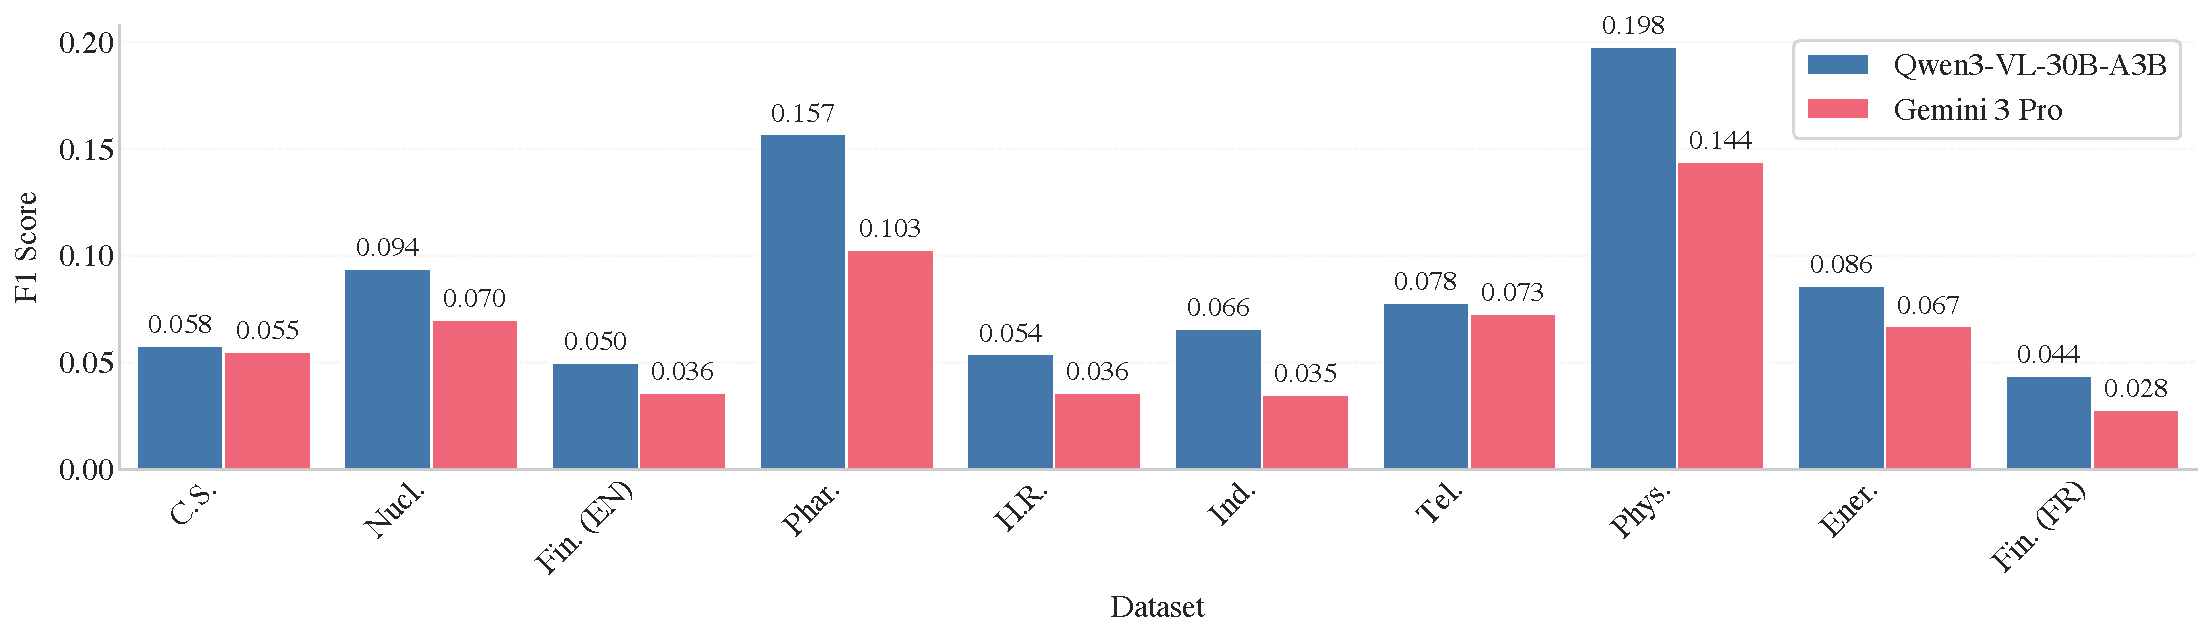
\includegraphics[width=\textwidth]{images/vidorev3_images/bbox_localization_by_dataset.pdf}
    \caption{\textbf{Model bounding box localization performance}. Each F1 score measures the zone-based overlap between model-generated bounding boxes and human annotations, using the annotator yielding the highest F1.} 
    \label{fig:bbox evaluation}
\end{figure*}

\section{Final answer evaluation} \label{appendix:final answer eval}

\paragraph{Evaluation setup} Generated final answers are evaluated in a pass@1 setting using GPT 5.2 with medium reasoning effort as the LLM judge. The judge compares each generated answer against the ground-truth annotation and returns a binary correctness label. The answer generation and judge prompts are shown in Figure~\ref{fig:generation_prompt} and Figure~\ref{fig:judge_prompt} respectively. We evaluated Gemini 3 Pro with low thinking effort, GPT-5 with medium reasoning effort, as well as the thinking version of Qwen3-VL-235B-A22B.

% To assess the variance of this evaluation, we conducted 5 independent runs on Gemini 3 Pro outputs using the oracle retriever with image context. Individual run scores were 71.72\,\%, 72.14\,\%, 72.14\,\%, 72.14\,\%, and 72.30\,\%, for a mean score of 72.09\,\% and a standard deviation of 0.22\,\% ((Krippendorff's $\alpha = 0.91$, indicating high intra-judge consistency).

To assess the reliability of our judge, we conducted 5 independent evaluation runs on a fixed set of Gemini 3 Pro outputs. Individual run scores showed minimal fluctuation (mean 72.09\,\%, $\sigma=0.22$\,\%) and high internal consistency (Krippendorff's $\alpha = 0.91$), confirming that the judge is consistent given a fixed context.

\paragraph{End-to-End Pipeline Stability} While the judge demonstrates high consistency on fixed inputs, the full evaluation pipeline introduces a second layer of variability: the model's generation process. To quantify the end-to-end variance under rigorous conditions, we performed 5 independent runs. For computational efficiency, we restricted this stress test to the most challenging corpus in each language: \textit{Industrial Maintenance} (English) and \textit{Finance} (French).

We measured an average score of 65.74\,\% with a standard deviation of 0.94\,\%. Crucially, the evaluation signal remains robust against generative noise, achieving a Krippendorff's $\alpha$ of 0.80. This agreement confirms that the end-to-end results are statistically reliable even when subjected to the most difficult evaluation scenarios.

\paragraph{Easy/hard query filtering} To classify queries by difficulty, we prompt a panel of 6 LLMs to answer each query without access to any corpus context. We select GPT-5-nano, GPT-5-mini, GPT-5, Qwen3-VL-30B-A3B, Gemini 2.5 Flash, and Gemini 2.5 Pro to span different model families and capability levels. Each model receives only the query text and is asked to provide a direct answer with the prompt in Figure~\ref{fig:easy_query_prompt}. Answers are evaluated for correctness using the same GPT-5.2 judge described above. A query is labeled \textit{easy} if at least one model answers correctly, and \textit{hard} otherwise. Table~\ref{tab: easy hard filtering} reports per-model accuracy and the resulting proportion of easy queries for each dataset. The distribution varies substantially across domains: knowledge-intensive datasets such as Computer Science and Physics have over 85\% easy queries, while domain-specific datasets such as Finance and Energy contain fewer than 35\% easy queries, reflecting the specialized nature of their content.


% \begin{table*}[h!]
% \centering
% \begin{tabular}{l c c c c c c c c >{\columncolor{avgcol}}c}
% \toprule
%  & \multicolumn{5}{c}{\textbf{English Datasets}} & \multicolumn{3}{c}{\textbf{French Datasets}} & \multicolumn{1}{c}{} \\
% \cmidrule(lr){2-6} \cmidrule(lr){7-9}
% \textbf{\# Queries} & C.S. & Fin. & Phar. & H.R. & Ind. & Phys. & Ener. & Fin. & \textbf{Total} \\
% \midrule
% Original    & 215 & 309 & 364 & 318 & 283 & 302 & 308 & 320 & 2419 \\
% Remaining   & 29  & 211 & 156 & 202 & 173 & 41  & 208 & 224 & 1244 \\
% \bottomrule
% \end{tabular}
% \caption{\textbf{\textit{Hard} query filtering statistics}. We report the original query counts versus the number of \textit{hard} queries remaining after filtering for model consensus.}
% \label{tab: hard queries answer generation}
% \end{table*}

\begin{table*}[h!]
\centering
\label{tab:performance_model}
% \resizebox{\textwidth}{!}{%
\begin{tabular}{l c c c c c c c c >{\columncolor{avgcol}}c}
\toprule
 & \multicolumn{5}{c}{\textbf{English Datasets}} & \multicolumn{3}{c}{\textbf{French Datasets}} & \multicolumn{1}{c}{} \\
\cmidrule(lr){2-6} \cmidrule(lr){7-9}
\textbf{Model} & C.S. & Fin. & Phar. & H.R. & Ind. & Phys. & Ener. & Fin. & Total \\
\midrule
GPT-5-nano     & 74.4 & 7.4  & 30.5 & 12.9 & 15.6 & 74.2 & 14.0 & 9.1  & 29.8 \\
GPT-5-mini      & 79.1 & 13.3 & 37.4 & 17.6 & 20.5 & 80.1 & 13.6 & 13.1 & 34.3 \\
GPT-5           & 76.3 & 25.2 & 50.8 & 29.9 & 32.2 & 80.5 & 26.0 & 22.2 & 42.9 \\
Qwen3-VL-30B-A3B & 60.9 & 3.9  & 19.2 & 6.3  & 9.9  & 60.9 & 6.8  & 4.4  & 21.5 \\
Gemini 2.5 Flash& 66.1 & 8.7  & 30.8 & 13.5 & 15.9 & 63.6 & 14.9 & 13.1 & 28.3 \\
Gemini 2.5 Pro  & 70.2 & 16.8 & 29.4 & 15.4 & 23.7 & 63.9 & 20.5 & 20.0 & 32.9 \\
\midrule
\textbf{Easy queries (\%)}           & 86.5 & 31.7 & 57.1 & 36.5 & 38.9 & 86.4 & 32.5 & 30.0 & 48.6 \\
\bottomrule
\end{tabular}
% }
\caption{\textbf{Percentage of queries correctly answered by LLMs without corpus context.} A panel of 6 LLMs is asked to answer the queries of the 8 public datasets without access to any corpus context. Queries correctly answered by at least one of the 6 models are classified as \textit{easy} queries, while the rest are labeled as \textit{hard}. Easy queries account for 48.6\,\% of all the queries.}
\label{tab: easy hard filtering}
\end{table*}


\clearpage

\section{Visual grounding examples}

% Merge of the 2 paragraphs below:

Qualitative analysis reveals distinct failure modes. Gemini frequently produces off-by-one page indexing errors: the predicted coordinates would correctly localize the target content if applied to an adjacent page. The two models also differ in box granularity: Gemini tends to draw tight boxes around individual elements (e.g., a single table cell or text line), whereas Qwen3-VL generates larger boxes encompassing entire sections or paragraphs, more closely matching human annotation patterns. Figures~\ref{fig:bbox examples qwen} and~\ref{fig:bbox examples gemini} illustrate these tendencies across four dataset pages: Qwen3-VL's bounding boxes are comparatively wide and encompass entire page elements (pages (a), (c), and (d)), while Gemini 3 Pro's visual grounding is more precise (pages (b) and (c)). This difference in granularity partially explains Qwen3-VL's higher F1 scores, as broader boxes are more likely to overlap with the ground-truth zones used in our evaluation. Both models exhibit errors and omissions: in page (b), the chart is not labeled by Qwen3-VL, and in page (d), Gemini 3 Pro predicts incorrect bounding boxes for the bottom table while Qwen3-VL provides grounding for the wrong table.

%Qualitative analysis reveals distinct failure modes. Gemini frequently produces off-by-one page indexing errors: the predicted coordinates would correctly localize the target content if applied to an adjacent page. The two models also differ in box granularity: Gemini tends to draw tight boxes around individual elements (e.g., a single table cell or text line), whereas Qwen3-VL generates larger boxes encompassing entire sections or paragraphs, more closely matching human annotation patterns \gmor{If we need to save some space for submission, these details about how Gemini and Qwen3-VL generates boxes could go to the Appendix}. This difference partially explains Qwen3-VL's higher F1 scores, as broader boxes are more likely to overlap with the ground-truth zones used in our evaluation.

%Figures~\ref{fig:bbox examples qwen} and~\ref{fig:bbox examples gemini} show examples of bounding box predictions by Qwen3-VL-30B-A3B and Gemini 3 Pro for 4 dataset pages. They show examples of the qualitative behavior of the models we observe throughout the dataset. Qwen3-VL's bounding boxes tend to be comparatively wide and encompass entire page elements, as seen in pages (a), (c) and (d), while Gemini 3 Pro's visual grounding is more precise (pages (b) and (c)). We also include evidence of errors and omissions from these two models: in page (b), the chart is not labeled by Qwen3-VL and in page (d), Gemini 3 Pro predicts wrong bounding boxes for the bottom table, while Qwen3-VL provides grounding for the wrong table.

\begin{figure*}[h!]
    \centering
    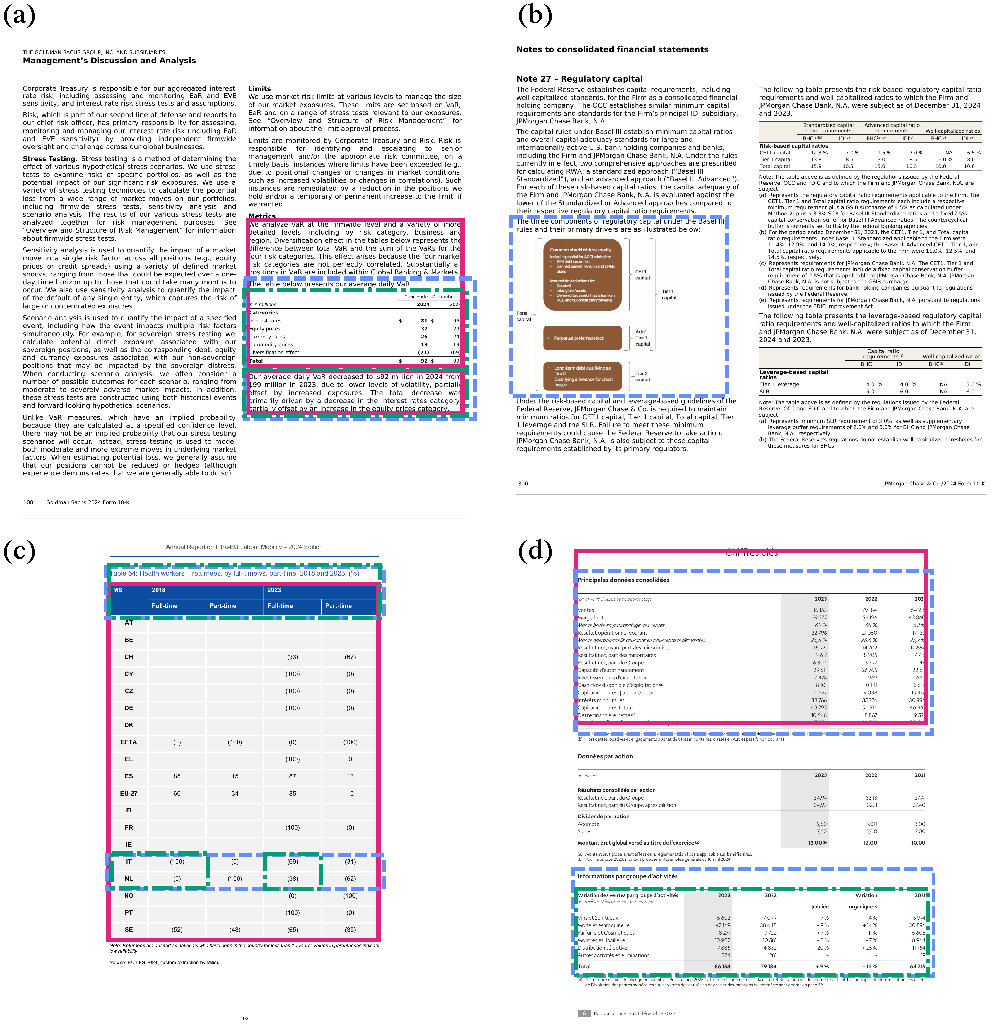
\includegraphics[width=\textwidth]{images/vidorev3_images/bbox_examples_qwen.pdf}
    \caption{\textbf{Visual grounding comparative examples for Qwen3-VL-30B-A3B.} Each panel shows a document page with Qwen3-VL's predicted bounding boxes (solid magenta) and human bounding boxes (dashed blue and green, one color per annotator). Corresponding datasets and queries: (a) finance\_en: What was the average daily Value at Risk (VaR) for Goldman Sachs during 2024?, (b) finance\_en: List the 3 components of regulatory capital under Basel III, and determine the role of each component., (c) hr\_en: Analyze how full-time employment among returning health workers evolved in the Netherlands and Italy from 2018 to 2023, and describe the differences in their employment trends., (d) finance\_fr: Croissance Mode Maroquinerie vs Vins Spiritueux 2023 performance}
    \label{fig:bbox examples qwen}
\end{figure*}

\begin{figure*}[h!]
    \centering
    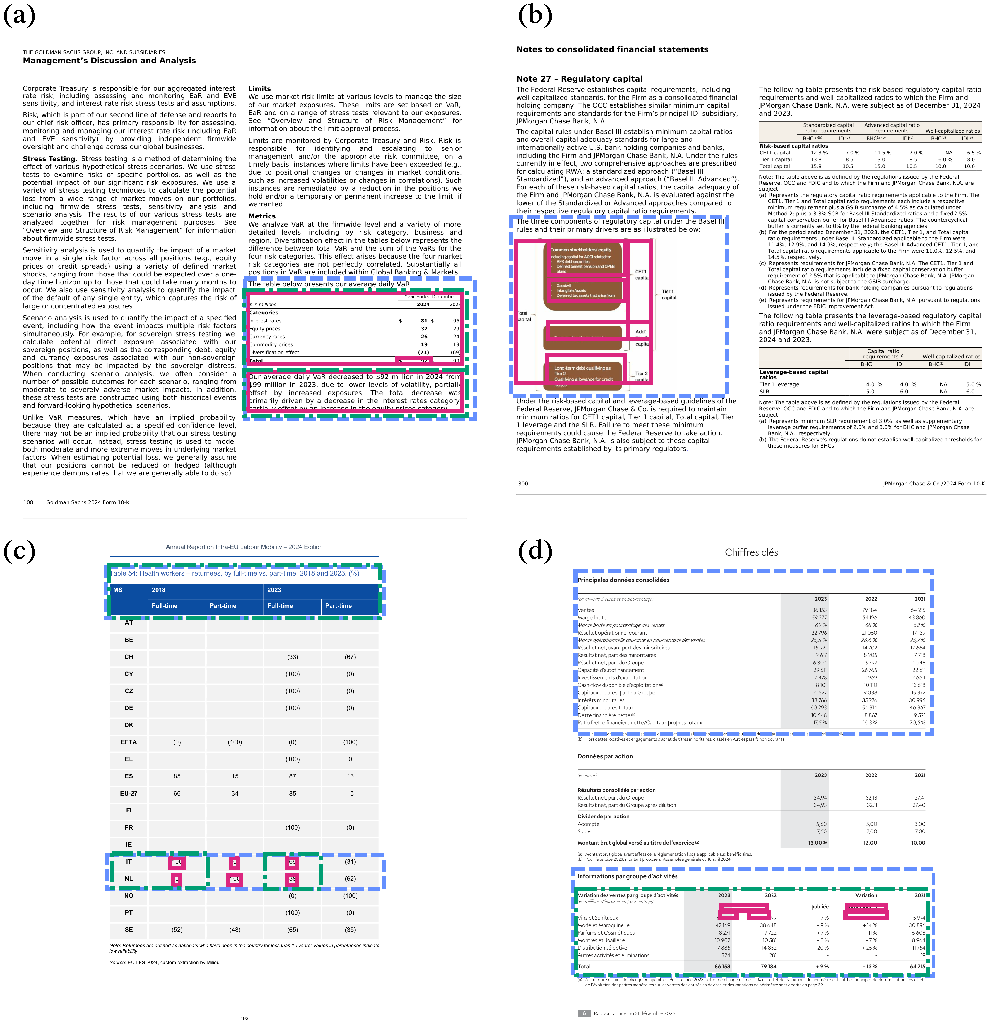
\includegraphics[width=\textwidth]{images/vidorev3_images/bbox_examples_gemini.pdf}
    \caption{\textbf{Visual grounding comparative examples for Gemini 3 Pro.} Each panel shows a document page with Gemini's predicted bounding boxes (solid magenta) and human bounding boxes (dashed blue and green, one color per annotator). Corresponding datasets and queries: (a) finance\_en: What was the average daily Value at Risk (VaR) for Goldman Sachs during 2024?, (b) finance\_en: List the 3 components of regulatory capital under Basel III, and determine the role of each component., (c) hr\_en: Analyze how full-time employment among returning health workers evolved in the Netherlands and Italy from 2018 to 2023, and describe the differences in their employment trends., (d) finance\_fr: Croissance Mode Maroquinerie vs Vins Spiritueux 2023 performance}
    \label{fig:bbox examples gemini}
\end{figure*}

\label{appendix: bbox examples}

% \clearpage

\section{Instructions given to Annotators}
\label{appendix: annotator_instructions}

\paragraph{Query Generation}\Cref{fig:task_1_instructions} details step-by-step instructions to annotators to generate queries from summaries and images.

\begin{promptfigure}[blue!5]{\textbf{Instructions given to human annotators to create queries}}{fig:task_1_instructions}
\begin{verbatim}
# Step 1
    The annotator will be provided with content(text summary or image(s)) and a list of instructions
    on the queries that are expected.

# Step 2
    Read and analyse the content.

# Step 3
    - The annotator writes a series of queries that can, supposedly, be answered by the summarized
    content. It is okay if the information needed to answer the question is in other parts of the
    document or not explicitly written in the summary.
    - If the summary is not adapted to a specific type or format of questions, the annotator may skip. 
    - They should follow the number of queries asked for each category.
    - They should follow the expected type of queries provided and the format.
\end{verbatim}
\end{promptfigure}


\paragraph{Query-Page Relevancy linking}\Cref{fig:task_2_instructions} details the step-by-step instructions provided to annotators for assessing page relevance, identifying content modalities, and localizing evidence via bounding boxes. \Cref{tab:relevance_scale} gives the definitions of relevancy scores used by the human annotators.

\begin{table}[h!]
\centering
\small
% Removed vertical bars (|) from the column definition
\begin{tabularx}{\columnwidth}{clX} 
\toprule
\textbf{Score} & \textbf{Label} & \textbf{Definition} \\
\midrule
2 & Fully Relevant & The page contains the complete answer. \\ 
\addlinespace % Adds a nice breathing room between rows without breaking lines
1 & Critically Relevant & The page contains facts or information required to answer the query, though additional information is required. \\ 
\addlinespace
0 & Not Relevant & Provides no information relevant to the query. \\
\bottomrule
\end{tabularx}
\caption{\textbf{Relevance definitions used for page-level annotations.}}
\label{tab:relevance_scale}
\end{table}

% \begin{table*}[h!]
% \centering
% \small
% \begin{tabular}{clp{7cm}}
% \toprule
% \textbf{Score} & \textbf{Label} & \textbf{Definition} \\
% \midrule
% 2 & Fully Relevant & The page contains the complete answer \\
% 1 & Critically Relevant & The page contains facts or information required to answer the query, though additional information is required \\
% 0 & Not Relevant & Provides no information relevant to the query \\
% \bottomrule
% \end{tabular}
% \caption{\textbf{Relevance scale used for page-level annotations.}}
% \label{tab:relevance_scale}
% \end{table*}

\begin{promptfigure}[blue!5]{\textbf{Instructions given to human annotators to annotate query-page relevancy}}{fig:task_2_instructions}
\begin{verbatim}
# Task overview
In this task, the annotator will be provided with a query and pages that are supposed to be relevant
to answer the query. The annotator’s goal is to rate the relevance in answerability of each page with
respect to the query.

# Step 1:
    - Review the query and pages to get an understanding of the content and domain
    
# Step 2:
    Rate the query quality. 
    - If adheres to guidelines > Good (1)
    - If doesn’t adhere to guidelines> Poor(0)
    - If the query is Poor quality, skip the task.
    
# Step 3:
    - For each page, rate the relevance with respect to the query
    - If page completely answer query > Fully Relevant(2)
    - If page contains information required to answer the query > Critically Relevant(1)
    - If page contains no relevant information > Not Relevant(0)
    
# Step 4:
    - For each page, annotate the modalities in which the relevant information is located concerning
    the query-page link, relevant information can be located in multiple modalities at the same time:
Modality : [“text”, “table”, “chart”, infographic”, “image”, “other”]
    - If relevance score = 0, modality may be “N/A”
    
# Step 5:
    - For each page, draw bounding boxes around the relevant text/chart/image/infographic (if any)
    - If relevance score = 0, do not draw a bounding box
    
# Step 6:
    - Repeat steps 3, 4 and 5 for all pages
    
# Step 7:
    - Propose an answer to the query, given the relevant pages.
    - If the query is not answerable, rate it as “unanswerable”

\end{verbatim}
\end{promptfigure}

\section{Prompts}

All the prompts used for both dataset generation and evaluations are detailed from \Cref{fig:query_generation_prompt} to \Cref{fig:bbox_instructions}.

\begin{promptfigure}{\textbf{Prompt used generate synthetic queries with the NeMo Data Designer tool}}{fig:query_generation_prompt}
\begin{verbatim}
<mission>
You are an assistant specialized in visual document understanding tasks. You will be given a context, 
summarizing the content of a section or multiple document sections. Your goal is to carefully analyze 
the context and to solve a series of tasks related to its content. You are tasked with generating 
query-answer pairs. Your queries will be used to simulate a user unfamiliar with the specific content 
of the page, and who is looking for information in a large knowledge base through a search engine. 
The user does not have access to the document and is looking for information that can be present in 
any document in the knowledge base.
</mission>

<definitions>
- A query is said to be fully answerable if the page contains a precise and complete answer to the 
query.
- A query is said to be partially answerable if the page contains relevant information that is 
directly related to the query but some key information is missing and must be retrieved in other 
pages or documents in order to give a precise and complete answer.
- An open-ended query is an explanatory or descriptive query that synthesizes  information; may be 
broad in scope and focused on qualitative aspects of the summary
- A compare-contrast query is a query that requires comparing and/or contrasting multiple entities or 
topics that are closely related to each other
- An enumerative query is a query that asks to list all examples that possess a common property, 
optionally requesting details about the specifics of each example.
- A numerical query is a query that asks for a specific number or calculated number given a summary. 
The query should require more than simply reading numbers directly from the page.
- A boolean query is a yes/no query that may involve multiple steps of reasoning.
- An extractive query is a clear and specific query that can be answered using only a specific piece 
of information.
- A multi-hop query is a complex query that requires retrieving and integrating information from 
multiple sources or steps to produce a complete answer.
- A question query is a complete sentence that ends with a question mark, typically used to seek 
specific information or clarification.
- A keyword query is a brief, often fragmented phrase or set of terms used to search or filter 
information, without forming a full grammatical sentence.
- An instruction query is a directive that describes a task to be performed on the documents, often in 
the form of a command or request.
</definitions>
<rules>
<queries>
- Generate queries only in {{ language }}.
- Make queries diverse, natural, and plausible for someone unfamiliar with the document.
- Each query must be standalone; do not reference “the page”, “the table”, “the figure”, 
“the document”, “the text”, “the table of contents”, etc.
- Rephrase; avoid copying wording from the source so semantic matching, not surface matching, 
is tested.
- You may include queries about relationships or trends often shown in images/vidorev3_tables/images/vidorev3_images/graphs, 
but never refer to a specific table/figure.
- Avoid overly generic queries that apply to any document.
- Keep each query concise ({{ length }} words).
- When appropriate, write multi-hop queries that integrate information across the provided pages.
</queries>
</rules>
<instructions>

Used Documents: {{ document_names }}
<summary>
{{summary}}
</summary>
Using the provided context, generate a {{ difficulty }}, {{ reasoning_type }}, {{ answerability }}
query. The query should be {{ query_type }} using the provided context and have the format of a 
{{ query_format }} query.
The query should be self-sufficient and related to the context.
</instructions>
\end{verbatim}
\end{promptfigure}

\begin{promptfigure}{\textbf{Prompt used to pre-filter the irrelevant pages for a given query}}{fig:query_linking_prompt}

\begin{verbatim}
<mission>
You are an assistant specialized in visual document understanding tasks. You will be given a document
page by page and a question. Your goal is to carefully analyze the page and say if it is related to
the question's answer. You are tasked with generating question-page affiliation as well as the
question answer if it exists in the page. 
</mission>

<definitions>
- A question is said to be fully answerable if the corresponding page contains a precise and complete
answer to the question.
- A question is said to be partially answerable if the corresponding page content is necessary to
answer the question but some key information is missing.
- A question is said to be unanswerable if the corresponding page contains information related to the
question's topic or domain but upon closer inspection does not contain information that is useful to
answer the question. Or if the page has no link whatsoever with the query.
</definitions>

<rules>
<page_affiliation>
- Be sure to put the relevance (and only that) between the tags <relevance>...</relevance>.
The possible values are: 
    <relevance>fully answerable</relevance>,
    <relevance>partially answerable</relevance>
    <relevance>unanswerable</relevance>.
- Be very careful when doing your page affiliation. Only say a page is relevant when it really is.
</page_affiliation>
<answers>
- You must generate the answer between the tags <answer>...</answer>. Between these tags, you should
only put the answer to the question.
- You must generate answers in the following language: {language}
- Your answers should be complete sentences.
- When the question is ambiguous, your answer should state that there is an ambiguity in the question.
- You should always generate the answer based on all the information available on the page, even if
the question was generated only on part of the page.
</answers>
</rules>

<instructions>
Return if the following question is "fully answerable" "partially answerable" or "unanswerable" based
on the content of the page between the tags <relevance> ... </relevance>. 
If the question is answerable, provide the answer.

Here is the question :
{{ query }}

And there is the page content :

</instructions>
\end{verbatim}
\end{promptfigure}

\begin{promptfigure}{\textbf{Prompt used to merge human annotators answers}}{fig:answer_merging_prompt}
\begin{verbatim}
You are given a set of document pages (images), a query, and a list of one or more
proposed answers.

Query :

{{ query }}

Proposed Answers:

{{ answers }}

Your task is to carefully analyze the provided pages, the query, and the proposed answers. You must
return a single, syntactically correct JSON object with the following structure:
```json
{
    "reasoning": "<string>",
    "information_in_pages": <true or false>,
    "answer_correctness": [<true or false>, ...],
    "reformulated_answer": "<string>"
}
```
Instructions for each field:
- reasoning: Explain the logic for each boolean in the `answer_correctness` list.
For each proposed answer, state why it is correct or incorrect, citing specific  evidence from the
document pages.

- information_in_pages: Set to `true` if the information needed to definitively answer the query
is present in the pages. Otherwise, set to `false`.

- answer_correctness: A list of booleans, corresponding to each proposed answer  in the original
order. Use `true` if the answer is verifiably correct based on the pages and `false` otherwise.

- reformulated_answer: A single string containing the most precise and correct answer to the query,
derived only from information in the pages. If any of the proposed answers are correct, use them as
a basis for synthesizing this improved answer. The reformulation must be concise and factual.

Important rules:
- Base your entire analysis strictly on the content of the provided document pages. 
Do not use outside knowledge.

- Do not invent, infer, or assume information that is not explicitly stated in the pages.

- Always provide a string for the `reformulated_answer`, even if no correct answer can be formed
from the text.

- Your final output must be only the JSON object.
\end{verbatim}
\end{promptfigure}

\begin{promptfigure}{\textbf{Easy/hard query filtering prompt}}{fig:easy_query_prompt}
\begin{verbatim}
Give a very precise and concise answer to the following query.
If you are unable to answer, output 'I don't know'.
Query: {{ query }}
\end{verbatim}
\end{promptfigure}

\begin{promptfigure}{\textbf{Judge prompt used for end to end evaluation}}{fig:judge_prompt}
\begin{verbatim}
You are an expert judge evaluating the accuracy of a test answer against a gold-standard true answer.
Your goal is to determine if the test answer captures the essential "core information."

### Evaluation Criteria:
- Correct: The test answer contains all core information of the true answer. Minor omissions of
non-essential details or the addition of minor, non-contradictory information should still be marked
as "Correct."
- Partially Correct: The test answer captures some of the core information, but suffers from
significant omissions or includes substantial extra information that was not requested or present in
the true answer.
- Incorrect: The test answer is fundamentally wrong, contradicts the true answer, or misses the core
information entirely.

### Input Data:
Query: {{ query }}

True Answer: {{ true_answer} }

Test Answer: {{ test_answer }}

### Output Format:
Provide a very brief explanation for your judgment. You must output your final response in a JSON
format with two fields: "explanation" and "judgment" (which must be "Correct", "Partially Correct",
or "Incorrect").
\end{verbatim}
\end{promptfigure}

\begin{promptfigure}{\textbf{Answer generation prompt used for end to end evaluation}}{fig:generation_prompt}
\begin{verbatim}
You are an expert at answering query based on documents.

Here is a list of relevant documents: {{ documents }}

Based on the above documents, answer the following query: {{ query }}

Keep the response short when appropriate. Output the answer only.
\end{verbatim}
\end{promptfigure}

\begin{promptfigure}{\textbf{Query translation from English to French prompt}}{fig:query_translation}
\begin{verbatim}
English text to translate: {{ query }}

Translate the English text above to French.
Make sure you follow the format of the English text. Don't change acronyms.
Follow the following json schema.
{
    "french_translation": ...
}
\end{verbatim}
\end{promptfigure}

\begin{promptfigure}{\textbf{Bounding box prediction prompt}}{fig:bbox_instructions}
\begin{verbatim}
# Role and Objective
- Serve as an expert in document analysis and visual grounding.
- Given a query and multiple document page images, provide a natural language answer with inline
grounding references.

# Instructions
- Analyze all provided pages to answer the query comprehensively.
- For each piece of information used in your answer, provide visual grounding by including bounding
box coordinates of all the sections of the document that help answer the query.
- Use this format to include the list of all bounding boxes of image N:
<bboxes image="N">[[x_{min}, y_{min}, x_{max}, y_{max}], ...]</bboxes>
  - image="N" specifies the 0-indexed page number (0=first page, 1=second page, etc.)
  - Include bounding boxes inline in your answer, immediately after mentioning the relevant
  information
  - A given page may contain multiple non-contiguous sections that help answer the query. In this
  case, you must output the list of the bounding boxes of all these sections.
  - You must group all the bounding boxes of a given page into a single 
    <bboxes image="N">...</bboxes> tag.

# Grounding Principles
- DO NOT output more than 5 bounding boxes per page.
- Adjacent logical units must be enclosed in a single, continuous bounding box.
- Return multiple bounding boxes only if information is clearly independent and separated by
significant non-relevant content.

# Output Format
- Provide a natural language answer to the query.
- Embed grounding tags directly inline where relevant information is discussed.
- Example: "The valuation technique described on page 1 
  <bboxes image="0">[[120, 450, 890, 670], [100, 800, 330, 960]]</bboxes> 
  uses discounted cash flow analysis."
\end{verbatim}
\end{promptfigure}
